% FEUP THESIS STYLE for LaTeX2e
% how to use feupteses (changed from the original for MIEEC)
%
% FEUP, JCL & JCF, Tue May 20 18:53:15 2008
%
% PLEASE send improvements to jlopes at fe.up.pt, jcf at fe.up.pt
%

%%========================================
%% Commands: pdflatex mieic
%%           bibtex mieic
%%           makeindex mieic (only if crating an index) 
%%           pdflatex mieic
%%========================================

%% For one side layout comment next line and uncomment the second line
\documentclass[11pt,a4paper,twoside,openright]{report}
%\documentclass[11pt,a4paper]{report}

%% For iso-8859-1 (latin1), comment next line and uncomment the second line
\usepackage[utf8]{inputenc}
%\usepackage[latin1]{inputenc}

%% Use option portuges if needed
\usepackage[portuguese,english]{babel}

%% For the final version, comment next line and uncomment the second line
\usepackage[alpharefs]{feupteses}      
%\usepackage[alpharefs]{feupteses} 

%% Options: 
%% - portuges: titles, etc in portuguese
%% - provisional: the thesis has not been approved yet
%% - usewatermark: use watermark instaed of provisonal text
%% - print: links are not shown (for paper versions)
%% - alpharefs: bibliography references are alphabetic
%% - numericrefs: bibliography references are numbered (in order of citation)
%% ( by default: author-date format of the ``natbib'' package is used 
%%   the portuguese version requires the file ``plainnat-pt.bst'' to be 
%%   present in the same directory )

%% Include MIEIC definitions different from standard style
\usepackage{mieicpatch}

%% Provide a version number in order to keep track of
%% thesis versions (it will printed in the footer of most pages)

\version{0.99}

%% Uncomment in the final version in order to make version footer disappear
\noversiontrue                 

%% Uncomment to create an index (at the end of the document)
%\makeindex                      

%% Path to the figures directory
%% TIP: use folder ``figures'' to keep all your figures
% \graphicspath{{figures/}}       

% For making gloassaries.
% http://en.wikibooks.org/wiki/LaTeX/Glossary
\usepackage[acronym]{glossaries}
\makeglossaries

%%----------------------------------------
%% TIP: if you want to define more macros, use an external file to
%% keep them
% Additional packages
\usepackage[utf8]{inputenc}
\usepackage{subfig}
\usepackage[pdftex,pdfpagelabels,bookmarks,hyperindex,hyperfigures]{hyperref}
\hypersetup{%
   plainpages=false, 
   pdfpagelayout=SinglePage,
   bookmarksopen=false,
   bookmarksnumbered=true,
   breaklinks=true,
   linktocpage,
   colorlinks=true,
   linkcolor=blue,
   urlcolor=blue,
   citecolor=blue,
   anchorcolor=green
}      

% There seems to exist some kind of standard on using CHapter with capital.
\def\chapterautorefname{Chapter}

\newtheorem{algorithm}{Algorithm}

% Based on: http://lists.cs.princeton.edu/pipermail/topic-models/2010-December/001081.html
% http://www.mpi-inf.mpg.de/~dietz/probabilistic-models-tikz.zip
% by Laura Dietz (dietz at mpi-inf.mpg.de)
%
\usepackage{color}
\usepackage{array}
\usepackage{verbatim}
\usepackage{float}
\usepackage{amsmath}
\usepackage{amssymb}
\usepackage{esint}

%%%%%%%%%%%%%%%%%%%%%%%%%%%%%% LyX specific LaTeX commands.
%% Because html converters don't know tabularnewline
\providecommand{\tabularnewline}{\\}
\floatstyle{ruled}
\newfloat{algorithm}{tbp}{loa}[chapter]
\floatname{algorithm}{Algorithm}

%%%%%%%%%%%%%%%%%%%%%%%%%%%%%% Textclass specific LaTeX commands.
\usepackage{float}
\floatstyle{ruled}
\newfloat{algorithm}{tbp}{loa}
\floatname{algorithm}{Algorithm}
\newfloat{genmodel}{h}{loa}
\floatname{genmodel}{Generative Process}
\usepackage[noend]{algorithmic}
\newcommand{\forbody}[1]{ #1 \ENDFOR}
\newcommand{\ifbody}[1]{ #1  \ENDIF}
\newcommand{\whilebody}[1]{ #1  \ENDWHILE}
\renewcommand{\algorithmicprint}{\textbf{draw}}

%%%%%%%%%%%%%%%%%%%%%%%%%%%%%% User specified LaTeX commands.


\usepackage{euscript}

\DeclareSymbolFont{rsfscript}{OMS}{rsfs}{m}{n}
\DeclareSymbolFontAlphabet{\mathrsfs}{rsfscript}


% PDF formatting instructions for A4
\pdfpagewidth=210mm % for pdflatex
\pdfpageheight=296mm % for pdflatex


%%%%%%%% begin tikz %%%%%%
\usepackage{tikz,tkz-base}
\usetikzlibrary{shapes,decorations,shadows}
\usetikzlibrary{decorations.pathmorphing}
\usetikzlibrary{decorations.shapes}
\usetikzlibrary{fadings}
\usetikzlibrary{patterns}
\usetikzlibrary{calc}
\usetikzlibrary{decorations.text}
\usetikzlibrary{decorations.footprints}
\usetikzlibrary{decorations.fractals}
\usetikzlibrary{shapes.gates.logic.IEC}
\usetikzlibrary{shapes.gates.logic.US}
\usetikzlibrary{fit,chains}
\usetikzlibrary{positioning}
\usepgflibrary{shapes}
\usetikzlibrary{scopes}
\usetikzlibrary{arrows}
\usetikzlibrary{backgrounds}


\pgfdeclarelayer{background}
\pgfdeclarelayer{foreground}
\pgfsetlayers{background,main,foreground}

\tikzset{latent/.style={circle,fill=white,draw=red,thick,inner sep=1pt, 
minimum size=20pt, font=\fontsize{10}{10}\selectfont},
obs/.style={latent,fill=gray!25},
const/.style={rectangle, inner sep=0pt},
factor/.style={rectangle, fill=red,minimum size=7pt, inner sep=0pt},
yellow/.style={latent,minimum size=15pt,fill=yellow!75},
blue/.style={latent,minimum size=15pt,fill=blue!75},
-/.style={color=red, thick},
>={triangle 45}}




% shapename, fitlist, caption, pos
\newcommand{\plate}[4]{
\node (invis#1) [draw, transparent, inner sep=1pt,rectangle,fit=#2] {};
\node (capt#1) [ below left=0 pt of invis#1.south east, xshift=0pt,yshift=-9pt] {\raisebox{0pt}[0pt]{\footnotesize{#3}}};
\node (#1) [draw=black!50,thick,inner sep=3pt,rectangle,rounded corners,fit=(invis#1) (capt#1),#4] {};
}


\newcommand{\shiftedplate}[5]{
\node (invis#1) [draw, transparent, inner sep=0 pt,rectangle,fit=#2] {};
\node (capt#1) [#5, xshift=2pt] {\footnotesize{#3}};
\node (#1) [draw,inner sep=2pt, rectangle,fit=(invis#1) (capt#1),#4] {};
}

%shapename, pos, caption, in1, in2, out, captpos
\newcommand{\twofactor}[7]{
\node (#1) [factor] at #2 {};
\node (capt#1) [#7 of #1]{\footnotesize{#3}};
\draw [-] (#4) -- (#1) ;
\draw [-] (#5) -- (#1) ;
\draw [->,thick] (#1) -- (#6);
}

%shapename, pos, caption, in, out, captpos
\newcommand{\factor}[6]{
\node (#1) [factor] at #2 {};
\node (capt#1) [#6 of #1]{\footnotesize{#3}};
\draw [-] (#4) -- (#1) ;
\draw [->,thick] (#1) -- (#5);
}

% name, --, caption, pos
\newcommand{\nofactor}[4]{
\node (#1) [factor, #2]  {};
\node (capt#1) [#4 of #1]{\footnotesize{#3}};
}

%shapename,  fitlist, caption
\newcommand{\namedgate}[3]{
\node (invisgate#1) [rectangle, draw, transparent,  fit=#2] {};
\node (gatecapt#1) [ above right=0 pt of invisgate#1.north west, xshift=-1pt ] {\footnotesize{#3}};
\node (#1) [rectangle,draw,dashed, inner sep=2pt, fit=(invisgate#1)(gatecapt#1)]{};

}

%shapename,  fitlist, caption
\newcommand{\gate}[3]{
\node (#1) [rectangle,draw,dashed, inner sep=2pt, fit=#2]{};
}

%shapename,  fitlist1, fitlist2, caption1, caption2
\newcommand{\vertgate}[5]{
\node (invisgateleft#1) [rectangle, draw, transparent,  fit=#2] {};
\node (gatecaptleft#1) [ above left=0 pt of invisgateleft#1.north east, xshift=1pt ]{\footnotesize{#3}};
\node (invisgateright#1) [rectangle, draw, transparent,  fit=#4] {};
\node (gatecaptright#1) [ above right=0 pt of invisgateright#1.north west, xshift=-1pt ] {\footnotesize{#5}};
\node (#1) [rectangle,draw,dashed, inner sep=2pt, fit=(invisgateleft#1)(gatecaptleft#1)(invisgateright#1)(gatecaptright#1)]{};
\draw [-, dashed] (#1.north) -- (#1.south);
}


\newcommand{\vertgateSpec}[5]{
\node (invisgateleft#1) [rectangle, draw, transparent,  fit=#2] {};
\node (gatecaptleft#1) [ above left=0 pt of invisgateleft#1.north east, xshift=1pt ]{\footnotesize{#3}};
\node (invisgateright#1) [rectangle, draw, transparent,  fit=#4] {};
\node (gatecaptright#1) [ above right=0 pt of invisgateright#1.north west, xshift=-1pt ] {\footnotesize{#5}};
\node (#1) [rectangle,draw,dashed, inner sep=2pt, fit=(invisgateleft#1)(gatecaptleft#1)(invisgateright#1)(gatecaptright#1)]{};
\draw [-, dashed] (#1.70) -- (#1.290);
}

\newcommand{\horgate}[5]{
\node (invisgateleft#1) [rectangle, draw, transparent,  fit=#2] {};
\node (gatecaptleft#1) [ above right=0 pt of invisgateleft#1.south west, xshift=1pt ]{\footnotesize{#3}};
\node (invisgateright#1) [rectangle, draw, transparent,  fit=#4] {};
\node (gatecaptright#1) [ below right=0 pt of invisgateright#1.north west, xshift=-1pt ] {\footnotesize{#5}};
\node (#1) [rectangle,draw,dashed, inner sep=2pt, fit=(invisgateleft#1)(gatecaptleft#1)(invisgateright#1)(gatecaptright#1)]{};
\draw [-, dashed] (#1.west) -- (#1.east);
}

\newcommand{\horogate}[5]{
\node (invisgateleft#1) [rectangle, draw, transparent,  fit=#2] {};
\node (invisgateright#1) [rectangle, draw, transparent,  fit=#4] {};
\node (#1) [rectangle,draw,dashed, inner sep=2pt, fit=(invisgateleft#1)(invisgateright#1)]{};
\node (gatecaptleft#1) [ above right=0 pt of #1.west, xshift=0pt ]{\footnotesize{#3}};
\node (gatecaptright#1) [ below right=0 pt of #1.west, xshift=0pt ] {\footnotesize{#5}};

\draw [-, dashed] (#1.west) -- (#1.east);
}


\newcommand{\vertogate}[5]{
\node (invisgateleft#1) [rectangle, draw, transparent,  fit=#2] {};
\node (invisgateright#1) [rectangle, draw, transparent,  fit=#4] {};
\node (#1) [rectangle,draw,dashed, inner sep=2pt, fit=(invisgateleft#1)(invisgateright#1)]{};
\node (gatecaptleft#1) [ below left=0 pt of #1.north, xshift=0pt ]{\footnotesize{#3}};
\node (gatecaptright#1) [ below right=0 pt of #1.north, xshift=0pt ] {\footnotesize{#5}};

\draw [-, dashed] (#1.north) -- (#1.south);
}


%%----------------------------------------

%%========================================
%% Start of document
%%========================================
\begin{document}

%%----------------------------------------
%% Information about the work
%%----------------------------------------
\title{Novelty Detection for Semantic Place Categorization}
\author{André Susano Pinto}
\degree{Master in Informatics and Computing Engineering}
%% Date of submission
\thesisdate{18 July, 2011}

%% Insert copyright text if used
%\copyrightnotice{Name of the Author, 2008}

\supervisor{Supervisor}{Andrzej Pronobis$^1$}{(Postdoctoral Researcher)}
\supervisor{Supervisor FEUP}{Luís Paulo Reis$^2$}{(Assistant Professor)}
\supervisornote{$^1$
  Centre for Autonomous Systems, The Royal Institute of Technology\\
  SE100-44 Stockholm, Sweden}{}
\supervisornote{$^2$
  LIACC - Artificial Intelligence And Computer Science Lab.\ of the University of Porto \\
  Rua Dr. Roberto Frias, s/n 4200-465 Porto, Portugal}{}

%% Uncomment committee stuff in the final version
\committeetext{Approved in oral examination by the committee:}
\committeemember{Chair}{António Fernando Vasconcelos Cunha Castro Coelho}{(Assistant Professor of FEUP\footnote{Faculdade de Engenharia da Universidade do Porto})}
\committeemember{External Examiner}{Luis Miguel Parreira Correia}{(Associate Professor of FCUL\footnote{Faculdade de Ciências da Universidade de Lisboa})}
\committeemember{Supervisor}{Luis Paulo Gonçalves dos Reis}{(Assistant Professor of FEUP$^1$)}
\signature
\committeedate{18 July, 2011}

%% Specify cover logo (in folder ``figures'')
\logo{figures/feup-logo.pdf}

%%----------------------------------------
%% Cover page(s)
%%----------------------------------------
\maketitle

%% Uncomment next line in the final version
\committeepage
%MIEEC uses an external PDF page with the signatures (juri.pdf)
%\includepdf[pagecommand={},noautoscale=false,fitpaper=true,pages=-]{juri.pdf}

%% Preliminary materials
\StartPrelim
\begin{singlespace}
  \chapter*{Abstract}

This should probably be written as last thing.

\chapter*{Resumo}
Let $E$ denote the set of all possible texts in English and $P$ the set of
all possible texts in Portuguese. A transformation $T_{E->P}(x)$ can be defined
in $E \times P$, such that it maps $x \in E$ to a translated version $y \in P$ such
that they hold the same semantic meaning to a reader.

Assume this text to be $T_{E->P}(abstract)$.
\footnote{What I mean is that this will be a translation of the english text present
on abstract and don't expect it to be filled in before the final version of this
document!}

 % the abstract
  \chapter*{Acknowledgements}
This thesis would have not been possible without the help of some other persons.
I would like to thank to Andrzej Pronobis, for introducing me to the problem and
directing it towards my interests in computer science, for the meetings, insights
and endless reviews of my work. Also to Carl Henrik Ek, for enthusiastically taking part
on the meetings discussing graphical models and related work.

The Computer Vision and Active Perception Lab at Royal Institute of Technology
in Stockholm were also a key piece for providing such a staff and facilities that
surrounded me during one year of thesis and exchange studies, and whose
courses replenish my interests in machine learning.
Also Faculdade de Engenharia of University of Porto who made it possible
for me to study and perform my thesis abroad.
Thanks to Luis Paulo Reis, for accepting to supervise my thesis and pushing me to submit a paper.

Virgile Högman, for besides handling me as a work colleague and chatter-box, becoming a friend.
And Erik Ass for all the interesting coding and math discussions on totally random problems.
I cannot also avoid to thank my neighbours back in Nockeby, in special to Diogo Gonçalves and Elise Löbker
that kept chatting with me through the nights during my thesis work.

Thanks to Mariatorget people who kept asking how my thesis was going and when it was going to be finished.
And for all the parties, drinking, relaxing and nights out! Thanks to Elina Säfsten, for being a cool neighbour
with whom I had the pleasure to spent quite some time talking and partying with her and her Swedish friends.
Thanks to Manuel Gattermayr and Tommaso Facchini for being awesome neighbours as well.

I am also grateful to Bernhard Schwaighofer, Manuel, Tommaso and others for an amazing
road trip, night fires, sunsets and sunrises on Sweden. Special thanks to Bernie for during the road trip
promising to wake me up before my sleeping bag starts to burn and melt with my skin and eventually turning me water proof.

And thanks to all the party people, not forgetting Andrzej, who showed me how to do a PhD party in case I ever decide
to seek one.

Last but not the least, thanks to my family and friends back in Porto and other parts of the world,
who kept talking and cheered me up.

% PS: This list does not contains all the persons the author of this thesis would like to thank, and the author should not be held liable for it.

\vspace{10mm}
\flushleft{
"I am thankful to all the awesome people who were part of this Stockholm chapter of my life"
--
\emph{André Susano Pinto}}

  % the acknowledgments
  %\cleardoublepage
\thispagestyle{plain}

\vspace*{8cm}

\begin{flushright}
   \textsl{``You should be glad that bridge fell down. \\
           I was planning to build thirteen more to that same design''} \\
\vspace*{1.5cm}
           Isambard Kingdom Brunel
\end{flushright}
    % initial quotation if desired
  \cleardoublepage
  \pdfbookmark[0]{Table of Contents}{contents}
  \tableofcontents
  \cleardoublepage
  % \pdfbookmark[0]{List of Figures}{figures}
  % \listoffigures
  % \cleardoublepage
  % \pdfbookmark[0]{List of Tables}{tables}
  % \listoftables
  % \cleardoublepage
  \pdfbookmark[0]{Glossary}{glossary}
  \printglossaries
  \cleardoublepage
  %\pdfbookmark[0]{Abbreviations}{abbrevs}
  %\chapter*{Abbreviations}
\chaptermark{ABBREVIATIONS}

\begin{flushleft}
\begin{tabular}{l p{0.8\linewidth}}
ADT      & Abstract Data Type\\
ANDF     & Architecture-Neutral Distribution Format\\
API      & Application Programming Interface\\
CAD      & Computer-Aided Design\\
CASE     & Computer-Aided Software Engineering\\
CORBA    & Common Object Request Broker Architecture\\
UNCOL    & UNiversal COmpiler-oriented Language\\
Loren    & Lorem ipsum dolor sit amet, consectetuer adipiscing
elit. Sed vehicula lorem commodo dui\\
WWW      & \emph{World Wide Web}
\end{tabular}
\end{flushleft}

  % the list of abbreviations used
\end{singlespace}

\newacronym{SVM}{SVM}{Support Vector Machine}
\newacronym{Dora}{Dora}{Dora: The Explorer}
\newacronym{CRFH}{CRFH}{Composed Receptive Field Histogram}
\newacronym{SIFT}{SIFT}{Scalar Invariant Feature Transform}
\newacronym{PCA}{PCA}{Principal Component Analysis}
\newacronym{K-PCA}{K-PCA}{Kernel Principal Component Analysis}
\newacronym{COLD}{COLD}{COsy Location Database}
\newacronym{MAP}{MAP}{Maximum a Posteriori}
\newacronym{KTH}{KTH}{Kungliga Tekniska Högskolan}
\newacronym{FEUP}{FEUP}{Faculdade de Engenharia da Universidade do Porto}
\newacronym{PLISS}{PLISS}{Place Labeling through Image Sequence Segmentation}


\newglossaryentry{ImageCLEF}
{
  name={ImageCLEF},
  description={is the cross-language image retrieval track which is run as part of the Cross Language Evaluation Forum}
}

\newglossaryentry{Kinect}
{
  name={Kinect},
  description={is a motion sensor introduced by Microsoft to create a controller-free gaming and entertainment experience. Since then it has been used by several researchers and hobbyist in the area of robotics}
}


%%----------------------------------------
%% Body
%%----------------------------------------
\StartBody

%% TIP: use a separate file for each chapter
% What should the title be?
% Novelty Detection for Visual Indoor Categorization
% Novelty Detection on Semantic Representations.

\chapter{Introduction}
\label{chap:introduction}

%\section*{}
%This chapter gives a generic overview of the problem, its motivation and goals. It also describes how the rest of the document is organized.

\section{Motivation}
There has been several efforts in the area of Artificial Intelligence and Robotics in creating robots that are able to interact with humans and their environments.
One of the existing problems is a reliable high-level localization method that can be deployed into new and unknown environments.

That task is specially difficult due to the constant change in those environments, either introduced by human interaction or by other external factors such as light-conditions.
Also the generalization requisite on such task requires highly generic and stable features to be extracted.

This thesis will focus on man-made indoor environments such as houses, offices, labs.
Where it would be desirable to map robot position to an high-level description such as kitchen, corridor, printer-area, office.
Such a classification can then be used to:
\footnote{Besides the motivation scenario, visual place classification has uses on other areas like augmented reality, content-base image retrieval and context awareness~\citep{dey2000towards}.}
\begin{itemize*}
\item Improve human interaction by mapping the robot localization to human concepts.
\item Improve robot localization methods with a high-level and robust localization information.
\item Extend knowledge about room categories and their properties.
\item Provide the robot with the ability to perform context-aware decisions.
\end{itemize*}

The robots should be able to operate in unknown environments as often they cannot be trained on the same environment they will operate on.
And under those circumstances the ability to distinguish between the known and unknown becomes a key point for reliability since it allows a robot to not trust the results it gets on new types of rooms.

It is therefore important to develop and access the quality of methods to identify novel cases.
Being the detection of novelty a key point for several tasks such as:
\begin{itemize*}
\item Operation in unknown environments.
\item Modelling what is know.
\item Ability to self-extend knowledge.
\end{itemize*}

\subsection{Visual features}
\label{sec:visual_motivation}
% Why Visual Place Classification!!
A robot often has several sensors that capture characteristics of its surrounding environment.
From those, vision is the most interesting and rich one and nowadays it is very easy to incorporate.
Making it a primary source of information for place classification.

Although its also the richness of the vision sensors that make it noisy and harder do interpret as the appearance of places varies over time due to illumination, human activity and view change.
It becomes then important to extract stable features from the visual input.
Visual features will be the main features explored during the thesis although other methods will also be used.

\section{Related Work}
\label{sec:related-work}
\cite{quattoni2009recognizing} showed that most scene recognition models work poorly in indoor scenes when compared to outdoor scenes results.
Since the properties that characterize rooms changes conforming its category. Namely corridors are well described by global properties and bookstores are well described by the presence of specific objects (books).
It became obvious then to use information provided by several sources. Their work uses both global and local features for scene recognition and does not address any specific information available in the context of mobile robotics.

This relation between room category and object has also been studied in the object search field.
Object search mainly focus on geometric properties but \cite{galindo2005multi} defines a bidirectional relation between object and room category, where object defines a room category and a room category provides information on where objects may be found.

Probabilistic representations are used in several localised functions in robots operating in the real-world~\citep{gross2009toomas,maierprobabilistic}. And some employ, up to some extent, a probabilistic representation across some subsystems~\citep{kraft2008exploration}.
\citet{vasudevan2008bayesian} performed room categorization through Bayesian reasoning about the presence of objects but did not included observations models (perception is considered deterministic).
And \cite{boutell2006factor} have studied outdoor scene classification using \emph{factor graphs} and modelling spatial relations between objects in the scene to extract better knowledge from semantic (high-level) features.

Its expected that using a unified probabilistic model from the whole system, such as \cite{pronobis2011exploiting}, more information can be reused to correctly predict a given random variable.

While there has been active research on visual properties and place classification, novelty detection applied to this problem has not seen much work on it~\citep{caputo2009overview}.
As \cite{markou2003novelty} reviews, novelty detection is an incredibly complex problem and requires specific techniques and methods to each problem.

\cite{bishop1994novelty} has showed that unconditional probability density can be use to provide a novelty measure. Though that probability is in most cases impractical to measure and even in those cases its necessary to find a correct threshold for \emph{novelty detection}. In higher-dimensions this method loses precision due to a spread out of the probability density function as most probability will be spread out on the tails of the function~\citep{markou2003novelty-part2}.

For that reason several other approaches have been developed for novelty detection.
One of those is the work of \cite{Hoffmann2007863} which applied non-linear statistical analysis to detect novel cases.
It has shown good results when applied to several problems such as digit recognition and cancer detection.

This type of approach although suffers from high computational and memory needs and often techniques need to be adapted to allow a online behaviour~\citep{sofman2010anytime}.


\section{Contribution/Goals}
\label{sec:goals}
During the thesis a thorough evaluation of a recently proposed property-based semantic mapping system for mobile robots~\citep{pronobis2011exploiting} on a real world visual database will be performed.

That system will be extended by usage of state-of-art novelty detection machine learning algorithms to the problem of visual place categorization.
As a final evaluation step, the developed method will be submitted to the Robot Vision Task on \gls{ImageCLEF}.

\section{Outline}
The rest of this technical report is organized as follows:

\begin{description}
\item[Chapter \ref{chap:background}] introduces the background for handling the presented problem.
It introduces the generic classification problem and techniques used to address it. Later developing on the specific visual features normally used as input for the place classification.

It also presents the novelty detection problem as well the techniques used to address it in the current context.

\item[Chapter \ref{chap:approach}] presents our approach to the problem. It introduces the platform over which the visual place classification is performed and points in the direction of extending such a platform for novelty detection.

\item[Chapter \ref{chap:testing}] introduces the testing and evaluation methodologies.
It also presents the databases used and the \gls{ImageCLEF} competition to which the developed work will be submitted.

\item[Chapter \ref{chap:workplan}] lists and elaborates on the planned tasks to be completed during the master thesis work and gives an estimated schedule for the working time. 
\end{description}



%%%%%%%%%%%%%%%%%%%%%%%%%%%%%%%%%%%%%%%%%%%%%%%%%%%%%%%%%%%%%%%%%%%%%%%%%%
%%%%%%%%%%%%%%%%%%%%%%%%%%%%%%%%%%%%%%%%%%%%%%%%%%%%%%%%%%%%%%%%%%%%%%%%%%
\chapter{Background}\label{chap:background}
% This chapter will perform a breath-first explanation on the contents related
% with the thesis. The extension of the contents explained here can be seen as
% monotone function over the number of missing pages to attain the requirements.
%
% Some topics are indeed important as its the case of factor graphs.
% Others like:
%  - classification (SVM, multi-class, kernel-trick),
%  - features (SIFT, GIST),
%  - Basic Bayes theory and probabilistic review
% are included for fun of the reader in case it inquires himself how to deal
% with the low-levels features we propose using.
%
% ---
% PS: This is the chapter that will be used to fill with unnecessary crap
% in case they really annoy me with the number of pages. Every other chapter
% will strive to be really required and be a masterpiece.
%

One of the interesting facts about high-level problems is that they often require a
broad overview of the whole system and several concepts. For example in the case of
this thesis approach to novelty detection on semantic knowledge it becomes first
important to understand how classification of already known categories is performed.
I.e.\ understand how can
lower\hyp{}level classifiers be represented, how to obtain those representations from
training data, and how to use those them to infer new classifications from those models.
It is also important to know how to model several of those classifications with
probabilistic relations in a unified model and how to infer information on those.

This chapter tries to briefly introduce the reader to those aspects. The presented material
is not complete, it serves only to give directions and cues to the reader on how the several
subproblems of visual place classification can be solved. 
Where appropriate it refers to articles or textbooks that present the introduced techniques.

\section{Classification}
Classification deals with the problem of identifying classes or groups that lie underneath
the sensed data. It is expected that the presence of a underlying concept is involved on the
generation of the data that is sensed, and the system tries to infer that underlying concept
without directly observe it.

Often the sensed data is just to large to be directly handled within a classifier. In those
cases classifiers work on a small subset of features extracted from the data. Those features
should avoid discard important information and if correctly employed should turn the classification
easier.

\subsection{Recognition and Categorization}
Classification can target very different types of classes, as it is not clear on which classes
the system is interested in distinguish. For example the system maybe interested in distinguish
specific instances or interested in detecting a wide group of instances matching a
common category. E.g. distinguish a specific room: room 304 in the 3rd floor, from a generic room
category: a library.

Based on the type of desired learning system, the available features and the required generalization
specifications a wide range of machine-learning methods can be used. And no single method
is expected to handle all the problems with optimal performance.
The methods can go from statistical classification, neural networks, nearest neighbours,
decision trees, support vector machines to others like graphical models, clustering,
Gaussian mixture models, hidden Markov models, principal component analysis~\cite{bishop2006pattern}.

This background chapter does not aims at describing all the classification methods, but at
introducing the concept of classifier and to use them to extract information from low\hyp{}level
features. In that sense only \glspl{SVM} will be generally described, for more information
on others the reader is welcome to check the vast literature in pattern recognition and machine
learning such as the standard textbook cited above.

\subsection{Supervised and Unsupervised Training}
It is often impossible to manually specify the information needed to correctly classify samples.
There is also interest to make systems flexible and allow them to learn and adapt based solely
on the available data. In that sense the option is to train classifiers from available data.
The training methods are often separated as:

\begin{description}
\item[Supervised Methods] assume the existent of a supervisor that is able to give the
ground\hyp{}truth. With it the algorithm tries to learn the best description that matches
the given labelled data.
\item[Unsupervised Methods] try to learn classes without any extra information. The methods
have to figure out how many and which classes seem more reasonable to be modelled.
\end{description}

\subsection{Discriminative and Generative Models}
\label{sec:discriminative-vs-generative}
After constructing a classifier from the information available either in form of
available knowledge on the task in hand and from acquired data samples, the agent
ends up with a model that represents the knowledge it believes to be suitable to
solve the task.

The produced model differs a lot based on the type of classifier but they can be
distinguished in two different categories:
\begin{description}
\item[Discriminative models] are only able to classify samples in the known categories.
\item[Generative models] model the full probability relation between sensed
features and classes. With that it becomes possible to use the learned model to generate
new samples.
\end{description}


\subsection{Multi-Class Classification}
\label{sec:multiclass-classifiers}
Most classifiers methods are designed as two-class classifier and do not
natively support multi-class classification problems.
The most common approach is to try to approach multi-class problems by
by combining several two-class classifiers and perform a voting scheme or other
integrating method based on the confidence of the individual two-class classifiers.
For example:

\begin{description}
\item[One Against All] - in this method $c$ distinct classifiers are trained to
distinguish any class of the remaining ones. The output of all those classifiers
(distance to the separating hyperplane) is then used to categorize the output.
The most common approach is to pick the class with the largest hyperplane
distance. Other variations exists as is the case of using the minimal distance
to the average classification distance of each class~\citep{pronobis2007iros}.

\item[One Against One] - in this method $c*(c-1)/2$ classifiers are trained to
distinguish between each pair of classes. The final decision is based on the
output of all those classifiers being common to use a majority vote strategy.
\end{description}


\subsection{Support Vector Machines}
\Glspl{SVM} where introduced by \cite{cortes1995support} and can be seen as
discriminative linear based classifier. They are based on a strong mathematical
foundation and have powerful generalization capabilities. In their original form
\gls{SVM} separates two classes of points in an hyper-space with a
\emph{maximal margin hyperplane}~(\autoref{fig:svm-sample}).
Later they were extended to deal with noisy data by using \emph{soft margins}.
And to handle non-linear spaces as seen on \autoref{sec:kernel-trick}.

\begin{figure}[h]
\begin{center}
% TODO: get a decent picture to illustrate SVMs
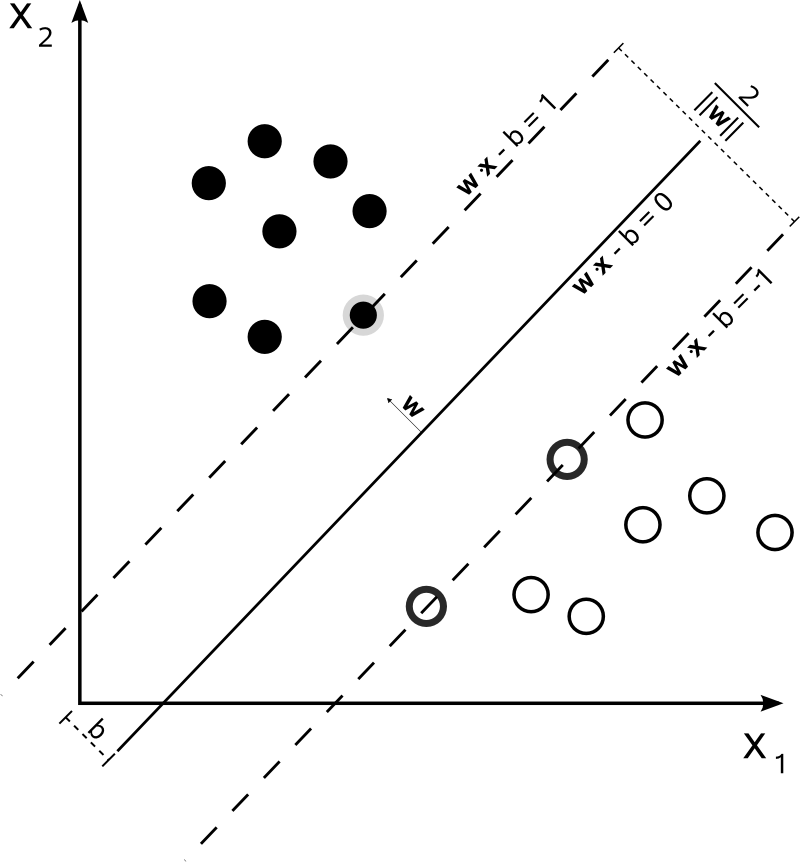
\includegraphics[width=0.4\textwidth]{figures/Svm_max_sep_hyperplane_with_margin}
\end{center}
\caption{{SVM} separating two class of points by a
         \emph{maximal margin hyperplane}. The hyperplane can be described by
         the collection of support vectors and associated weights, marked in the
         image as sample points with large borders.}
\label{fig:svm-sample}
\end{figure}

They have been used in several classification and recognition problems and are
in fact a standard across machine learning techniques. Their efficiency, exact
training results and generalization made them suitable for many tasks. Such as
text categorization, digit-recognition, spam-classification.
They have also been extensively used in visual place classification.
% TODO: add citations.

\subsection{Kernel-Trick}
\label{sec:kernel-trick}
Several classifiers can be modelled by requiring only the concept of inner\hyp{}product
between two samples. That product is often seen as a measure of distance or similarity
between the samples on some space. By using kernels it becomes possible to define such
space without explicit convert the samples to it. By abstracting the concept of distance
on such a kernel function it also becomes possible to use those classification methods
on strange data structures such as trees, strings or graphs.

For example \glspl{SVM}, in their basic form, are only able to handle linear spaces.
But the classes are most of the time not linearly separable in the input
space. Although there might exists a transformation $\phi$ from the original
space into a space $H$ where the input becomes linearly separable.

The Kernel trick allows to extend the \gls{SVM} definition to work on such space
$H$ without ever performing an implicit transformation between spaces. Being
enough for that to have a Kernel function defining an inner-product inside such
space: $K(x_i, x_j) = \phi(x_i)\cdot\phi(x_j)$.

Several kernel functions have been proposed being the most commonly used:

\begin{description}
\item[Polynomial Kernel] - $K(x, y) = (x \cdot y + p)^d$
\item[Radial Basis Function] - $K(x, y) = e^{-\gamma\|x - y \|^2}$
\item[Histogram Intersection] - $K(x, y) = e^{-\gamma \chi^2(x,y)}$, where
$\chi^2(x,y) = \sum_{i=1}^{N}\frac{(x_i-y_i)}{x_i+y_i}$ introduced by
\cite{barla2003histogram} allows to compute histogram similarity.
\item[Matching Kernels] - mimic matching similarity and are used when each
sample is represented as a set of features~\citep{boughorbel2005intermediate}.
\end{description}


\section{Features}
A feature is a piece of information which is expected to reveal information for
solving a specific task. Features are task-dependant and they will
yield different performance based on the type of task they are applied to.

A wanted property on features is its repeatability under similar conditions for
the problem in hand. This is: they should be stable and invariant across
unwanted types of transformations and noise. For example a visual feature for
object detection should be present even if the target object was translated,
scaled, rotated, the light-conditions have changed or even if the object is
partially occluded.

Extracting features with those properties allows to greatly reduce the size of
input by removing unwanted noise and useless information from the captured data.
Turning the classification problem easier, more reliable and more efficient.

Often several and different types of features need to be extracted. It has been
reported by \cite{pronobis2010ijrr} that using multiple features provides a
great benefit in the context of place classification.
And \cite{quattoni2009recognizing} has showed that different types have
different impact in indoor scene recognition based on the type of scene
matching. Specifically it was seen that some room-categories are more likely to be
recognized by the presence of some objects and others by it generic appearance.

In the context of robotics, sensors such as cameras, laser scans are used to
sense the surrounding environment, and features can be extracted from those.
Visual features can be seen as belonging to two categories:
\emph{local features} and \emph{global features}.


\subsection{Local Features}
\label{sec:local-features}
Local features describe fine grain properties of a part of image.
For example the existence of specific corner or an edge. \Gls{SIFT}
is an example of such feature and it been proven useful
for matching points between images and subsequence extension to object detection.

\subsubsection*{Interesting Points and SIFT}
\label{sec:sift}
The detection of interesting points has been studied for several years and is
the base of several computer vision problems solution. It allows to perform
point matching which can be used in several areas from image stitching,
3D reconstruction, video tracking, object detection, etc\dots

The most used method was presented by \cite{lowe1999object}. And its based on
building a feature vector for each image. Each of those features is based on
\emph{interesting points} detected by detecting maxima and minima of a
difference of Gaussian functions applied in a scale-space.
The scale space is used to provide scale invariant detection. Gaussian functions
are used as they are the only way to model a linear scale-space.
Each interesting point is then described by a container that is rotation
invariant.

By seeing an object as a set of features points, index and matching is then
performed by a high-dimensional search on a database of know objects. After
matching objects can be verified for geometric coherence between features.
\Gls{SVM} classifiers can also be trained to detect objects based on this type
of local features by using \emph{Matching kernels} (\autoref{sec:kernel-trick}).

\begin{figure}[h]
    \centering
    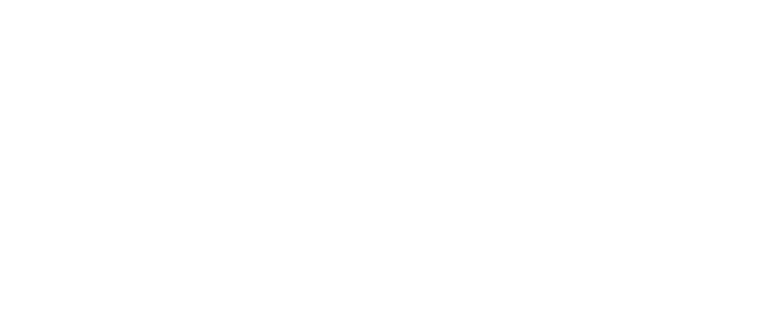
\includegraphics[width=0.8\textwidth]{figures/sift/sift.pdf}
    \caption{{SIFT} and other local features have been proven useful in object
             detection.}
\end{figure}


\subsection{Global Features}
Global features try to describe the whole image. E.g.\ either by
statistical analysis of features over all the image or by a structured
distribution of textures findable in the image.

\subsubsection*{Gist of a Scene}
\label{sec:gist}
\cite{oliva2006building} argue that fast scene recognition does not need to be
built on top of object recognition but can be analyzed by scene-centered
mechanisms.
They defend that position by pointing out behaviours on human vision:
when provided with a glance of a shot a person can identify the meaning of that
given shot or "gist of a scene" without remembering specific details.

As seen on \autoref{fig:gist} the gist is able to capture the dominant textural
features of the overall image and their coarse spatial layout~\citep{murphy2006object}.
With that, it is expected they serve the purpose of correctly describe the image
textures without the need to directly stored the original image.

\begin{figure}[h]
\center
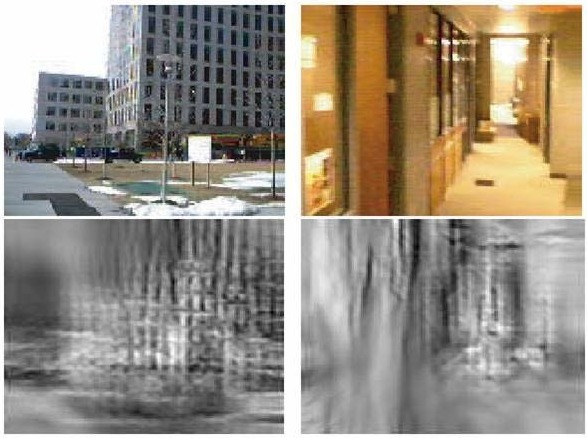
\includegraphics[width=0.60\textwidth]{figures/gist.jpg}
\caption{\label{fig:gist}An illustration of the gist of an image. Top row: original image I;
         bottom row: noise image J for which gist(I) = gist(J).}
\end{figure}


\subsubsection*{{CRFH} - Composed Receptive Field Histograms}
\label{sec:crfh}\label{sec:global-features}
\gls{CRFH} are a multidimensional statistical
representation of the occurrence of several image descriptors applied to an
image. They can be seen as an high-dimension histogram where each cell records
how many pixels of the image have the cell response for the applied descriptors.
Such high-dimensional histogram is expected to be able to describe global
information contained in the image by capturing several properties that co-occur
in a part of the image.
By using some techniques~\cite{linde2004object} several operations on those
high-dimensional histograms can be made computational efficient. This way not
only this descriptor discards part of the local information present on the image
but also allows to faster computations on similarity measures.


\begin{figure}[h]
\begin{center}
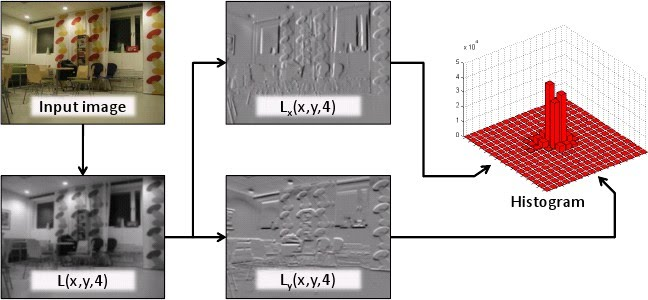
\includegraphics[width=1\textwidth]{figures/crfh_model.jpg}
\end{center}
\caption{A two dimensional histogram of the image built out from two image
         descriptors: $Lx$ and $Ly$. First-order Gaussian derivatives of image
         luminance in horizontal and vertical direction applied at a scale 4.}
\end{figure}

Multidimensional histograms have proven to be useful in the context of object
recognition~\citep{schiele1996object}. And have also been previously used in
the context of visual place classification~\cite{pronobis2010ijrr}.
\emph{Histogram intersection kernels} (\autoref{sec:kernel-trick}) can be used
to train classifiers based on this feature.


%%%%%%%%%%%%%%%%%%%%%%%%%%%%%%%%%%%%%%%%%%%%%%%%%%
% Important sections of this chapter begin here.
%%%%%%%%%%%%%%%%%%%%%%%%%%%%%%%%%%%%%%%%%%%%%%%%%%
\section{Probability Theory}
An important aspect when making decisions with noisy or missing information is
the uncertainty of the received information and of the final conclusion.
Probability theory comes to help by providing a framework able to deal with those
issues~\cite{bishop2006pattern}.

The key concept on it is that of \emph{probability}, which can be seen as way of
express the degree of belief that a certain event occurs.
When combined with decision theory it allows to perform optimal decisions with the
available information, even if it is ambiguous or incomplete.

A probability $P(x)$ of a given event $x$ is a value between $0$ and $1$, where $0$ means
the belief that $x$ will not occur and $1$ that it will certainly occur.
In cases $x$ does not specifies all the variables states that define the sample space, $P(x)$
is called a marginal probability. 

Often it is impossible to exactly describe the probability of a given event, in such cases
the concept of likelihood comes to help.
The likelihood of an event only has meaning when compared to one of another event.
In such case the ratio between both likelihoods will denote on how more likely an event is
over another.
When dealing with discrete and countable sample spaces any likelihood function can be converted
to a probability function by calculating the normalization factor such that the sum over all
the sample space is $1$.

\subsection{Conditional Probability}
It is also possible to denote the known information when calculating probabilities. For that
the notion of conditional probability is used $P(a|b)$. It denotes the probability of $a$
knowing that $b$ has occur. Often conditional probability is also represented by: $P_b(a)$.
In this thesis both notations will be used: the former for representing the information on
sensed variables and the second for representing information or assumptions on other generic
information such as graph structures.

Marginal probabilities can be related with conditional probabilities as described in the equation:
\begin{equation}
P(a|b) P(b)  = P(a, b)
\end{equation}


\section{Principle of Maximum Entropy}
\label{sec:max-entropy}
The principle of maximum entropy~\cite{shore1980axiomatic} states that when given
a set of distributions that are coherent with the acquired knowledge, the one which
maximizes entropy should be picked.

This can be used to select a distributions that most correctly describes the obtained
knowledge. For example, if all that is known from a distribution is the mean and deviation
then the correct approach is to model it with a normal distribution with the known parameters.
In case of having no information available, the uniform distribution shall be assumed.


\section{Probabilistic Graphical Models}
\label{sec:graphical-models}
% THIS IS ALL JUNK TEXT COPIED
Graphical models usage can be tracked back to earlies 1920 but they only become
popular in mid-eighties when researchers started to use \emph{Bayesian Networks}
to model expert systems~\citep{borgelt2002graphical}.

They serve as a better tool to model \emph{random variables}
(nodes on the graph) and their probabilities as they model the conditional
dependence between variables (edges on the graph). Important to note that here
\emph{random variables} does not denotes a truly random variable but one that is
unknown by the system and is conditioned by other variables/evidences.

This type of graphs provide a generative model where the probability of any
given scenario can be determined.
This means once a graphical model is learned, it can be used to generate new
samples from the learned distribution.

They have been successfully used in several machine-learning task such as:
information extraction, speech recognition, computer vision.
They are also useful due to their ability to deal with semantic (high-level)
features~\citep{boutell2006factor} and ability to represent properties of the
reality they try to model.

Two main types of graphical models are widely used: Bayesian Networks which model
directed edges between variables and Markov Random Fields where variables are
connected by a potential but no special direction is given to edges.

An important property of these graphs is the \emph{Markov-blanket} of a node.
For a given variable $a$, a \emph{Markov-blanket} is a set of variables in the
surroundings of $a$ that when given the value of $a$ becomes independent of the
rest of the graph~\citep{pearl1988probabilistic}.
On non-directional graphs it is directly determined by the nodes connected to $a$.
This allows the usage of graph algorithms such as \emph{min-cut} to quickly
determine most likely scenarios. In the case of directed edges a node blanket is
also influenced by the direction of the edges and more complex schemes need to
be used.

As \cite{lauritzen2002chain} points this two types of models can be represented
as a \emph{chain graph} where both directed and undirected edges can co-exist.
Though this generalization is hard to implement due to mis-understandings on the
concepts the graph-models use.

Another useful interpretation of graphical-models are \emph{factor graphs}.
Those are able to handle both \emph{Bayesian Networks} and
\emph{Markov Random Fields}. Under this interpretation a graph is seen as a
bipartite graph that connects variables with factors that influence
them~\citep{bishop2006pattern}.
This gives a very useful framework to develop belief propagation on them by
seeing a message-passing mechanism between nodes. Belief propagation is used to
calculate marginal-probabilities.

\begin{figure}[ht]
\centering

\subfloat[Bayes Networks] {
  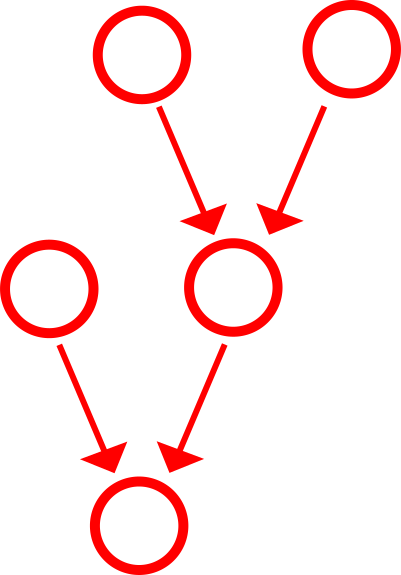
\includegraphics[width=0.2\textwidth]{figures/graphical-models/BayesNet.pdf}
}
\quad
\subfloat[Markov Random Field] {
  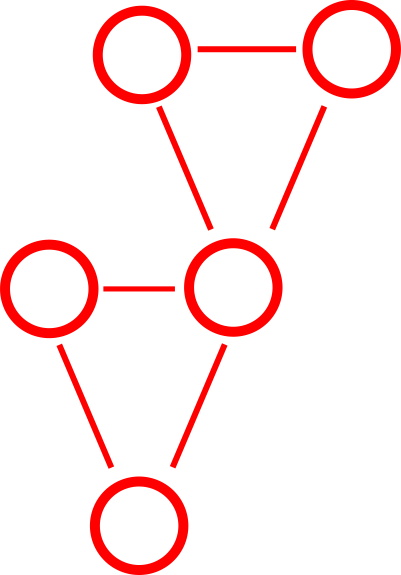
\includegraphics[width=0.2\textwidth]{figures/graphical-models/MarkovRandomField.pdf}
}
\quad
\subfloat[Factor Graph] {
  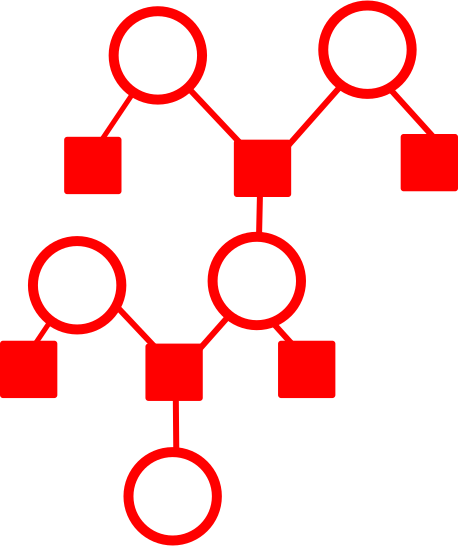
\includegraphics[width=0.3\textwidth]{figures/graphical-models/FactorGraph.pdf}
}
\end{figure}

\subsection{Factor Graphs}
A \emph{factor graph}~\cite{kschischang2001factor} is a bipartite graph connecting two sets of nodes $X_G$ and $F_G$
representing random variables and factors.
Each factor is described by function $\phi$ dependent only on the variables $x_\phi$
to which the factor is connected.
Thus, a factor graph can be seen as a description of probability density function obtained
by a product of all the factors. In order to represent the probability,
a normalization factor needs to be introduced, resulting in the following equation:

\begin{equation}
P_G(x) = \frac{1}{Z}\prod_{\phi \in F_G}{\phi(x_{\phi})},\qquad
Z = \sum_{X_G}\prod_{\phi \in F_G}{\phi(x_{\phi})}
\end{equation}

\subsection{Inference}
The goal by obtaining a graphical model between all the variables of a system is the ability
to efficiently infer the most likely scenarios based on the available information.
The sensed information can be used to clamp variables and the model used to calculate probabilities
or marginal probabilities.

In that sense a basic operation on a graph is the \gls{MAP} operation, which allows to calculate
which configuration on a variable or subset of variables maximizes a given function.


%%%%%%%%%%%%%%%%%%%%%%%%%%%%%%%%%%%%%%%%%%%%%%%%%%%%%%%%%%%%%%%%%%%%%%%%%%
%%%%%%%%%%%%%%%%%%%%%%%%%%%%%%%%%%%%%%%%%%%%%%%%%%%%%%%%%%%%%%%%%%%%%%%%%%
\chapter{Semantic Mapping}\label{chap:semantic-mapping}

% motivation
Humans associate concepts to areas that relate to the functionality of those. That
association is either useful by explaining where to find certain objects as well to
understand the types of activities to perform on it. In a 

Those human-concepts are meant to be meaningful for humans and by incorporating conceptual
knowledge about them it is expected to improve the agent 
% semantic mapping definition
In this context semantic mapping is seen as the process of building a representation of
the environment which associates spatial entities with a set of defined spatial concepts (i.e.\ human concepts).

% importance of conceptual knowledge
% application of conceptual knowledge
It is expected that by being able to reason over those semantics an agent can better
understand human environments and increase its efficiency when performing human-tasks on them.
By handling this conceptual knowledge the agent becomes aware of 


% challenges and need for representing uncertainty
The goal of a spatial representation is to provide the agent with a view about the environment
that allows it to reason beyond its sensory horizon.

 Such a representation is by its nature
imperfect, incomplete, inaccurate and invalid.

world that allows the agent to perform reasoning over it and efficiently perform tasks.
It should also give the agent ability to reason about parts 
Such a representation cannot be perfect since the methods and information are uncertain

% here a here a method is used that does semantic mappping and representes conceptual knowledge
% on a probabilistic fashion.



It is therefore clear that the need to handle information on an high-level semantic and
probabilistic fashion arises not only for efficiency reasons but also from the desire
of being able to communicate and reason on those aspects.
In order to fully explore the semantic properties and their relations it is necessary to
detect and classify semantic aspects as well to understand the relationships between them.
That conceptual knowledge is important and any limitations on it will limit the capacities
of an agent to reason. 

This thesis motivation lies on developing methods for detecting knowledge gaps
on the semantic knowledge of a mobile agent. For that the semantic mapping system
implemented on \gls{Dora} proposed by \cite{pronobis2011phd} was used as a base.


\section{Architecture Overview}
Pronobis~\cite{pronobis2011phd} presents a system architecture working in indoor environments using
non\hyp{}omnidirectional laser and visual sensors for semantic mapping. The system integrates cues such as geometry,
object presence and appearances and is able to perform inference across any semantic properties,
for example for the purpose of place categorization.
The introduced system is built around a spatial knowledge representation~\cite{pronobis2010ias} and it has not only been tested on real-scenarios
and performance tested across several conditions~\cite{pronobis2007iros} but also shown
to be tailored to effectively solve tasks arising on mobile robotics~\cite{hanheide2011ijcai}.

Besides that the spatial knowledge representation has been drawn with an high-focus on probabilistic
and uncertain reasoning, human interaction and life-long learning capabilities.
For that it was considered an excellent base defining not only the concepts and
requirements of an high-level semantic representation but also the information flow
between all the layers involved on the agent.

Being able to perform probabilistic inference on all available information Such a representation is suitable to detect novel concepts.


The system is implemented on \Gls{Dora} and a brief overview of its architecture is
given in the following sections.

\section{Spatial Knowledge Representation}
\cite{pronobis2010ias} proposes a spatial knowledge representation sub-divided into four layers.
Each layer focus on different aspects of the world, abstractions levels of the spatial knowledge
and different spatial scales. Each uses different spatial entities and relate to the agent
goals in different ways:

In the lowest abstraction level the sensory layer represents the most immediate and short term
accurate representation of the world. Above, the place layer discretizes the continuous
space into. The categorical layer focus on knowledge of low\hyp{}level, long\hyp{}term
categorical models of the sensory information. And at the higher level the conceptual map
associates concepts to areas such as rooms (see \autoref{fig:spatial-knowledge}).

\begin{figure}[h]
\centering
\includegraphics[width=0.7\textwidth]{figures/spatial-knowledge-representation.pdf}
\caption{\label{fig:spatial-knowledge}Layered structure of the spatial representation.}
\end{figure}

\subsection{Sensory Layer}
The sensory layer keeps a detailed representation of the immediate surrounds of the agent.
That representation is based on directly sensed inputs as well on data-fusion for short
time\hyp{}intervals.

It is responsible for providing the agent with an exact position and to accurately position
low\hyp{}features and landmarks. The information is stored with associated uncertainty it
is highly susceptible to be replaced with newer versions. Also old or distant information
is forgotten.
By tracking the surrounds for short amount of times it provides an accurate representation
that can be used to locate and guide the agent on low\hyp{}level movements.

\subsection{Place Layer}
The place layer is responsible for maintaining a bottom\hyp{}up discretization of the
continuous space. On it the world is represented as a collection of discrete spatial
entities, called places, together with connectivity information.

Each place is defined with the features from the sensory layer and with spatial relations
to other places. Connectivity here, stands for ability to travel directly between the
places. Additionally places can be created for areas not yet explored allowing to introduce
virtual place holders to places that would eventually be uncover if the agent moved there.

The places are also considered stable on long\hyp{}term and can be used to help the agent
performing localization and planning longer distance motion planning. This higher level
representation although uncertain allows to model connectivity and relaxed spatial relations.

\subsection{Categorical Layer}
The categorical layer holds the generic long-term, low-level representations of categorical models
of the agent's sensory information.
The knowledge represented by this layer is not instance specific. It is the knowledge
required to determine certain features indicate the presence of an entity of certain
category. E.g.\ the knowledge required to detect objects, landmarks or describe room appearances.
Other properties may as well be defined for example shape, color, edges and size properties
are all defined in terms of low\hyp{}level features.

This layer is responsible for representing knowledge on how to extract properties used
by the conceptual layer.
Although not mandatory, in many cases the categories represented by it will map to human concepts
and not to the internal concepts of the agent.
The type of properties handled by this layer may require incredible complex models and for
that they might be trained on a supervised fashion.

\subsection{Conceptual Layer}
The conceptual layer provides an ontology that represents a taxonomy of the spatial concepts
and their relations with the properties represented on the categorical layer.
This associates semantic meaning to those properties that is useful for human-agent iteration
and provides relations that can be verbalized and explained with the ontology.

It provides also knowledge between the semantic concepts and their instances of those concepts.
Including definitions of spatial concepts related to space segmentation as well to semantic
categorization of those spatial entities.
E.g.\ rooms are commonly split by doors, rooms exist in a floor, a building has floors, milk is
likely to be found on kitchens, etc\dots

By providing information for segmentation, semantic mapping to concepts and relations between those
concepts, the knowledge represented on this layer allows the agent to explain and reason close to
the human concepts. The knowledge represented here is considered to be valid through very long
periods of time or even life\hyp{}long.


\section{System Structure}
The \Gls{Dora} system~\cite{hanheide2011ijcai} consists of several co-operating
sub-systems~(see \autoref{fig:dora-architecture}),
all of which actively use or maintain the \emph{spatial knowledge representation}.

The layer structure of the spatial knowledge representation allow to implement
data driven processes that control the flow of knowledge and information between the
lower and higher\hyp{}levels layers. To reduce computation and make it feasible not
all updates from lower\hyp{}levels are treated immediately. Instead the system waits
until a substantial change has occurred.

\begin{figure}[h]
\centering
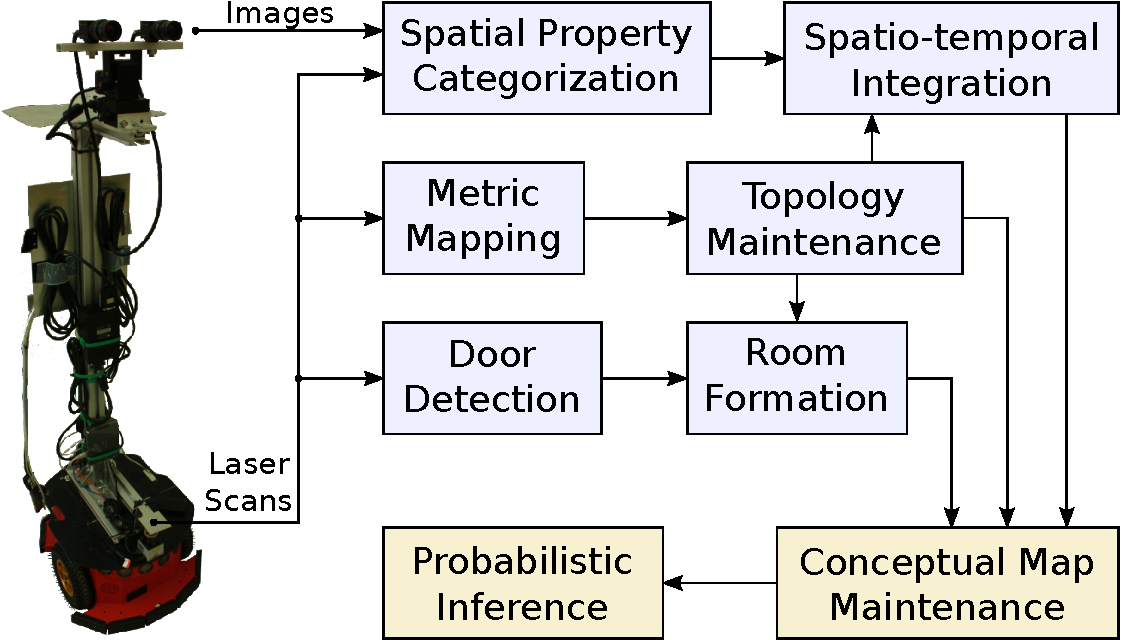
\includegraphics[width=0.8\textwidth]{figures/dora-architecture.pdf}
\caption{\label{fig:dora-architecture}Dora the Explorer as well as the elements and the data flow inside
         the semantic mapping system.}
\end{figure}

Initially the low-level topology and metric mapping systems use a \gls{SLAM} algorithm~\cite{Folkesson07a}
that is used as representation on the sensory layer. Those two systems are also responsible
for creating the place map on the place layer, as that is highly related with the \gls{SLAM} goals.
By using the landmarks (doors) and other available information the system also tries to
group places and understand the concept of rooms.

At the same time the spatial property categorization system is responsible for detecting
instances of the categorical knowledge by running classifiers previously trained to detect
a set of features listed on \autoref{sec:dora-features}. For that it uses the data available
from a laser range finder and a camera and besides classifying the features it estimates also
its confidence on the information.
The extracted features together with the estimates is then integrated over time and space
in order to increase its robustness.

Finally the conceptual map system utilizes the acquired instance knowledge together with
the high\hyp{}level conceptual knowledge to create a probabilistic graphical model that allows
to run inferences.
Since this conceptual mapping processing is responsible for creating the probabilistic
graphical model it is described in detail in \autoref{sec:conceptual-map}.


\subsection{Features}
\label{sec:dora-features}
The \emph{categorical layer} requires classifiers with the ability to categorize the
low\hyp{}level features into categories.
For that \gls{Dora} performs detection on the following categorical entities:
\begin{description}
\item[Doorway Detection] by using the laser range finder the system tries to detect doors.
\item[Geometric Shape] by using features extracted from the laser data and pre-trained classifiers
the system tries to classify rooms according to their shapes (e.g.\ rectangular, square).
\item[Geometric Size] is classified once again recurring to laser data. In this case the system
\item[Object Detection] is performed by running traditional object recognition classifiers.
Those are previously trained on a supervised fashion to later be able to detect objects
based on their visual features, e.g.\ by using \gls{SIFT} as described in \autoref{sec:sift}.
tries to categorize the room size according to a set of previously learned concepts (e.g. large, medium, small).
\item[Visual Appearance] is extracted from the visual input. For that Dora uses a trained
a set of classifiers on global visual features such as \gls{CRFH} to categorize the visual
appearance of a room in categories such as corridor, office, library.
\end{description}

\section{Conceptual Map}
\label{sec:conceptual-map}
As \gls{Dora} moves through the environment it builds a \emph{conceptual map}: a structural and
probabilistic representation of the space instantiated as a \emph{graphical model}.
It includes taxonomy of human\hyp{}compatible spatial concepts which are linked to the sensed 
instances of these concepts drawn from lower layers. It is the conceptual layer which 
contains the information that kitchens commonly contain cereal boxes and have certain 
general appearance and allows the robot to infer that the cornflakes box in front of the 
robot makes it more likely that the current room is a kitchen. The conceptual layer is 
described in terms of a probabilistic ontology defining spatial concepts and linking 
those concepts to instances of spatial entities (see the example of the ontology in
\autoref{fig:spatial-knowledge}).

Based on this design, a \emph{chain graph} model is proposed as a 
representation for performing inferences on the knowledge represented in the conceptual 
layer. Chain graphs are probabilistic graphical models that combine the properties of 
both Bayesian Networks and Random Markov Fields. This results in an efficient approach to 
probabilistic modeling and reasoning about conceptual knowledge.

\begin{figure}[h]
\centering
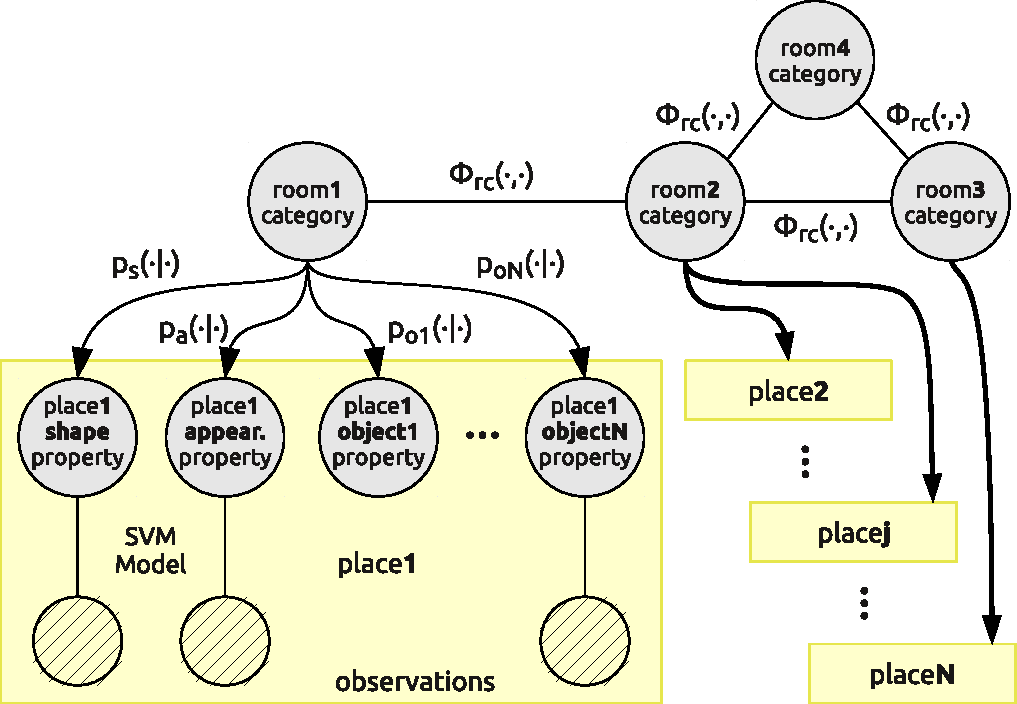
\includegraphics[width=0.75\textwidth]{figures/chaingraph.pdf}
\caption{\label{fig:chain-graph}Example chain-graph instantiated from the \emph{conceptual layer}.}
\end{figure}

%The conceptual layer structures the sensed environment together with the conceptual knowledge
%in order to create a structured probabilistic representation of the world.
An exemplary chain graph corresponding to the conceptual map ontology is presented
in \autoref{fig:chain-graph}. 
Each discrete place identified in the environment is represented by a set of random variables, 
one for each class of relation linked to that place. These are each connected to a random variable
over the categories of rooms, representing the ``is-a'' relation between rooms and their categories. 
Moreover, the room category variables are connected by undirected links to one another according 
to the topological map. The remaining variables represent: shape and appearance properties of space 
as observed from each place, and the presence of objects. 
These are connected to observations of features extracted directly from 
the sensory input. Finally, the 
distributions $p_{s}(\cdot|\cdot)$, $p_a(\cdot|\cdot)$, $p_{o_i}(\cdot|\cdot)$ 
represent the common sense knowledge about shape, appearance, and object co-occurrence, respectively. 
They allow for inference about other properties and room categories e.g. that the room is likely to be a kitchen,
because you are likely to have observed cornflakes in it. 

The use of graphical models to describe distributions of variables has useful properties.
First, they permit inference about uncertain conceptual knowledge. At the same time, they are 
generative models and therefore allow to calculate the probability
on any given subset of variables of the graph, allowing the system to work even when some
information is missing.

\subsection{Factor Graphs}
Although the conceptual layer works with \emph{chain graphs}~\cite{lauritzen2002chain},
those can be converted into \emph{factor graphs}~\cite{kschischang2001factor}.
Factor graphs have been introduced in \autoref{sec:graphical-models} and are used
throughout this thesis as they provide an easier manipulation due to factorization.

Moreover, there exist efficient implementations of inference engines operating on factor
graph representations~\cite{Mooij_libDAI_10}.
Describing the distribution function in terms of graphs permits the use of those engines to
efficently calculate marginals on any given subset of variables by exploiting conditional
independence between variables.

\subsection{Uncertain Sensing and Implicit Factors}
\label{sec:cues-from-low-level}
In a realistic scenario, classification tasks are by their nature uncertain.
And although a trained classifier is able to decide which class is more likely, there is
interest in handling uncertainty produced by those to make decisions more robust.

By modelling the classifiers as an implicit function $\phi_{classifier}(c, x)$ it becomes
possible to model the uncertainty of the decision given the presence of the sensed low-level
features $x$. The presence of those implicit models no longer allow calculation of the
normalization factor over the whole graph as there is no explicit model for either the
low\hyp{}level features $X$ (e.g.\ $X$ can be an image received from a visual sensor)
or for $\phi_{classifier}$ (e.g.\ the classifier can be an \gls{SVM}).

Nonetheless it is still possible to calculate any probability given that the features $X$
are observed. For that instead of modelling the variables $X$ and explicitly describing
the factor $\phi_{classifier}$ it is enough to replace it by an observed factor
$\phi_{classifier}(c|x)$ as shown on \autoref{fig:implicit-factor}.


\begin{figure}[h]
\centering
\subfloat[]{
\begin{tikzpicture}
  \node [matrix,matrix anchor=mid, column sep=20pt, row sep=10pt,ampersand replacement=\&] {
    \& \& \node (graph) [] {\dots}; \& \& \\
    \& \& \node (prop) [latent] {$c$}; \& \& \\
    \& \& \node (fac) [factor] {}; \& \& \\
    \& \& \& \& \\
    \node (x1) [obs] {$x_1$}; \&
    \node (x2) [obs] {$x_2$}; \&
    \node (x3) [obs] {$x_3$}; \&
    \node (xi) [] {\dots}; \&
    \node (xn) [obs] {$x_n$}; \\
  };
  \draw [-] (prop) -- (graph);
  \draw [-] (prop) -- (fac);
  \draw [-] (fac) -- (x1);
  \draw [-] (fac) -- (x2);
  \draw [-] (fac) -- (x3);
  \draw [-] (fac) -- (xi);
  \draw [-] (fac) -- (xn);

  \node (captfactor) [right=2pt of fac] {\footnotesize{$\phi_{classifier}(c, x)$}};
\end{tikzpicture}
}
\qquad
\subfloat[]{
\begin{tikzpicture}
  \node [matrix,matrix anchor=mid, column sep=20pt, row sep=10pt,ampersand replacement=\&] {
    \& \& \node (graph) [] {\dots}; \& \& \\
    \& \& \node (prop) [latent] {$c$}; \& \& \\
    \& \& \node (fac) [factor] {}; \& \& \\
    \& \& \node (hidden) [latent,draw=none] {}; \& \& \\
  };
  \draw [-] (prop) -- (graph);
  \draw [-] (prop) -- (fac);
  \node (captfactor) [right=2pt of fac] {\footnotesize{$\phi_{classifier}(c | x)$}};
\end{tikzpicture}

}

\caption{\label{fig:implicit-factor}By modelling classifiers as implicit factors it is
possible to perform inference on the graphical models handling the uncertainty measures
produced by those classifiers.}
\end{figure}



%%%%%%%%%%%%%%%%%%%%%%%%%%%%%%%%%%%%%%%%%%%%%%%%%%%%%%%%%%%%%%%%%%%%%%%%%%
%%%%%%%%%%%%%%%%%%%%%%%%%%%%%%%%%%%%%%%%%%%%%%%%%%%%%%%%%%%%%%%%%%%%%%%%%%
\chapter{Novelty Detection}\label{chap:novelty-intro}

This chapter presents the main work of this thesis: a method to augment the conceptual
map with novelty detection capabilities.

The chapter starts by providing the reader with a brief overview on novelty detection
techniques and related works. Then it shows that an optimal novelty detection system
can be implemented by thresholding an order relation defined over the inputs.
Moreover, an equivalent order relation can be imposed by a ratio between
conditional and unconditional probabilities.

Finally,  a practical example using semantic data and probabilistic graphical
models is presented: it shows how to use the introduced ratio to obtain a
novelty detection system and analyses the performance impact by increasing
the amount of sensed data and by using an approximation on the unconditional
probability.


\section{Novelty Detection - Review and Related Work}
Novelty detection, also known as outlier or anomaly detection, is a
classification problem related to identification of new or unknown data
patterns that the system is not aware of~\cite{markou2003novelty}.

The ability to identify novel cases is crucial in any autonomous system
that is deployed to unknown or to uncontrolled environments, as it gives the
system the ability to detect that something is not conforming to its knowledge and
therefore should be treated with caution.
It has several applications such as fault detection~\cite{tarassenko1999novelty},
intrusion detection~\cite{fan2001using},
detection of masses in mammograms~\cite{tarassenko1995novelty} or detection of
novel and useful documents~\cite{zhang2002novelty}.

Any normal classification application is also a good candidate for extending
with novelty detection, as the results for samples on which the system has not been
trained on can be unreliable~\cite{devarakota2008reliability}
e.g. when applied to digit-recognition~\cite{tax1998outlier}
or to detection of novel inputs on a neural network~\cite{bishop1994novelty}.

It is in the nature of unknown environments and in the infeasibility of
the system to acquire examples of all possible classes where the complexity of
novelty detection lies: it is only possible to obtain samples representing positive
examples of known cases and the lack of negative examples renders normal
classification methods unusable.
In order to become practical in real world applications, novelty detection
methods have to overcome a series of obstacles:
be able to generalize while still detecting novelty,
be resistant to noisy features,
scale in feature dimension,
deal with multiple classes and perform detection efficiently as many
autonomous systems require real-time or close to real-time performance.

\subsection{Review of Novelty Detection Methods}
A common approach is to use density estimation and use the expected probability
of a sample to classify the sample as novel. Examples of such techniques are
Gaussian Mixture Models and Parzen-window estimators. In order to be effective,
those rely on data as close as possible to the input features and use
dimensionality\hyp{}reduction techniques such as \gls{PCA} to make density
estimation feasible. Note that as dimension increases an exponential number
of data samples would be required to approach the density with the same quality.

\cite{bishop1994novelty} uses that approach by employing a Parzen-window to
estimate the density of the training data on a given input fed into a
neural-network. Using the calculated density, they detect samples
that differ from the training data and consider their neural-network output
to be unreliable as the samples are distinct from what the network was trained
with.

A slightly different approach is applied in case of by one-class \gls{SVM} approaches that
try to distinguish novelty by separating the training set from all the other
points in the input space. This is achieved by enclosing the training
set with some structure (e.g.\ an hyper-sphere)~\cite{bennett2000support}.
Those approaches have been made in line with Vapnik's principle of never to solve a 
problem which is more general than the one we actually need to solve~\cite{scholkopf2000support}.
Although having access to a perfect probability distribution
of the input would solve the problem, creating such a function is harder than
simply creating a boundary between known data and novel data.

Error reconstruction methods have also been used for novelty detection.
They use the assumption that the class to be defined lies on a manifold embedded
into a sample space of higher dimensionality. By using dimensionality\hyp{}reduction
techniques, a manifold is defined and the distance between the manifold and the new sample
is calculated. One of the most common methods used for that purpose is
\gls{K-PCA}~\cite{scholkopf1997kernel}, which uses the kernel-trick to extend
\gls{PCA} and perform a nonlinear dimensionality reduction of the input.
This technique has been successfully used for novelty detection in \cite{Hoffmann2007863}.

\cite{japkowicz1995novelty} also follows a similar approach: \emph{Redundancy
Compression and Non-Redundancy Differentiation} which is a process believed
to happen in the hippocampus. They introduce an auto-encoder
that learns to encode a sample on a considerable smaller description and later reconstructs
the original sample from this smaller description. Their suggested system
learns how to discard and compress redundant information while still be able to recover
the original sample. By training it with samples from a given class, it
is expected that it will badly reconstruct a sample from a different one.

\cite{ranganathan2010pliss} presents a system able to perform place recognition
and classification from visual clues. It is able to perform segmentation by
exploiting time-coherency on video information. The approach is particularly
interesting by its ability of keep a fully probabilistic distribution of
the place classification and segmentation. In other words, the system never performs
a deterministic decision that impacts any future result, allowing it to adjust
the segmentation and place classification as more data becomes available.
The system is also able to detect novel instances and methods how to adapt it
to run on a constant amount of memory and computation are presented.

\cite{boutell2006factor} presents a method to perform scene-classification
from low-level region detectors using probabilistic graphical models.
The information obtained by the region detectors is exploited together with the
spatial relations for the higher level scene-classification task.
A scheme using only pairwise relations between regions is shown to
have better performance than the correct approach of modelling connectivity of all regions 
with a large single factor as the pairwise relations can be
approximated with modest amounts of training data, where the single factor
demands an impractical amount of training data.
No approach is made for novelty detection either of the regions or the scene
categories. 


\section{Novelty Detection by Thresholding}
\label{sec:threshold}
The objective of a novelty detection system is to classify a given sample $x$ as
either \emph{known}: $x$ being generated by a class known to the system, or \emph{novel}:
$x$ generated by a class unknown to the system. Based on the ground\hyp{}truth of a sample four cases are possible:

\begin{description}
\item[true positive]  - when a system correctly   flags a sample of an unknown class as \emph{novel}.
\item[false positive] - when a system incorrectly flags a sample of a known class as \emph{novel}.
\item[true negative]  - when a system correctly   flags a sample of a known class as \emph{known}.
\item[false negative] - when a system incorrectly flags a sample of an unknown class as \emph{known}.
\end{description}

Due to noisy data, unstable features and lack of information, it is impossible to develop
a method able to always exactly guess the correct classification of a sample.
By modelling the outcomes with probabilities, it becomes possible to handle the uncertainty
associated with each decision.
The notation $P(novel|x)$ will be used to denote the probability that the sample $x$ is in fact a
sample of an unknown class. $P(x)$ will denote the probability that sample $x$ is given to the
system to be classified. $\overline{novel}$ is also defined in such a way that
$P(\overline{novel}|x)$ measures the probability that the sample $x$ is generated by a known class.

Additionally a decision on the novelty of a sample $x$ performed by a deterministic system
will be fully determined by the sample itself.
Which implies that any deterministic novelty detection system can be uniquely determined by the set $N$
of samples that are accepted by the classifier as \emph{novel}.
This way it is possible to define the probability of a true positive and false positive event for any
deterministic novelty detector with the following equations:

\begin{eqnarray}
P(\text{true positive})  &=& \sum_{x \in N}{P(novel|x)P(x)} \\
P(\text{false positive}) &=& \sum_{x \in N}{P(\overline{novel}|x)P(x})
\end{eqnarray}

Note that since probability functions are non-negative, it is impossible to decrease either the
true positive or the false positive probability by using a set $N' \supset N$.
This describes the base of the \emph{error and rejection tradeoff}~\cite{chow1970optimum}, which
states that a system aiming at increasing the true-positive probability will eventually increase its
false-positive error.
The true positive probability is related to the goal of detecting as many novel samples as possible.
At the same time, the false positive probability is related to the goal of not making too many errors.
By fixing one of those, it is possible to define a novelty detection system that achieves the maximum or minimum of the other.

This way an optimal detector can be formulated by achieving the maximum true-positive
probability without its false-positive probability increasing beyond a given limit.
This is equivalent to a \emph{continuous knapsack problem} which allows a greedy
solution by sorting the items with a value per weight function. In the case of 
detection system that can be defined as:

\begin{eqnarray}
value(x)  &=& P(\text{true positive}|x) \\
weight(x) &=& P(\text{false positive}|x) \\
cost(x)   &=& value(x)/weight(x) \\
          &=& \frac{P(novel|x)P(x)}{P(\overline{novel}|x)P(x)}
\end{eqnarray}

Therefore a novelty detection system before classifying a sample $a$ as novel should (greedily)
classify any sample $b$ with a smaller cost as that would achieve a higher true positive probability 
given a fixed false positive one.

\begin{equation}
\label{eq:knapsack}
\frac{P(novel|b)}{P(\overline{novel}|b)} < \frac{P(novel|a)}{P(\overline{novel}|a)}
\end{equation}

This relation between $a$ and $b$ can further be simplified into:

\begin{equation}
P(\overline{novel}|b) < P(\overline{novel}|a)
\end{equation}


Based on this, it can be said that an optimal novelty detection system is
interested in defining an order relation on all the possible inputs equivalent
to the order defined by the function: $P(\overline{novel}|x)$.
And any optimal detector can be described by the largest $P(\overline{novel}|x)$
accepted by it. This can be seen as thresholding.


\section{Conditional and Unconditional Probability Ratio}

In the previous section, it was shown that an optimal novelty detector can be
implemented by placing a threshold on the order relation defined by
$P(\overline{novel}|x)$ over $x$. Performing some manipulations with
Bayes theorem and assuming a constant $P(\overline{novel})$, a more usable
form can be attained:

\begin{equation}
\label{eq:novelty-ratio}
          P(\overline{novel}|x)
  =       \frac{P(x|\overline{novel}) P(\overline{novel})}{P(x)}
  \propto \frac{P(x|\overline{novel})}{P(x)}
\end{equation}

Since the interest is only in maintaining the order relation defined by
$P(\overline{novel}|x)$, any constant factor can be dropped.
Leaving a ratio between a \emph{conditional} and
\emph{unconditional probability} suitable for implementing novelty detection
by thresholding.


\subsection{Conditional Probability}
The conditional probability $P(x|\overline{novel})$ describes the distribution
of the samples given that they are generated by a known class.
In case when the labelled data used to learn a concept come from
the same distribution from the test samples come, the correct approach is to use it
as prior information for modelling the conditional probability.

Note that it is important for the labelled data to be a filtered version
of the underlying world distribution (one modeling all the concepts in the world) 
that does not contain any bias. Otherwise that bias will lead to incorrect modelling of 
the conditional probability and in consequence wrong ordering of the sample space.

\subsection{Unconditional Probability}
The unconditional probability $P(x)$ plays an important role in obtaining a
correct order relation for performing novelty detection.
It serves as a normalizing component that allows the system to decide
whether conditional probability of a given sample arises from it belonging to
the known concept or from the likelihood of being sampled.

On lack of any information about the unconditional probability and conforming to
the principle of maximum entropy (\autoref{sec:max-entropy}) a uniform
distribution must be chosen. However, by using unlabelled data, it becomes possible 
to obtain extra information and achieve a better approximation.


%\subsection{Novelty Detection on a Variable Set of Features}
Note also that often novelty detection is applied to a fixed set of features
together with an assumption of a uniform unconditional probability.
In those cases, $P(x)$ becomes a constant and therefore a novelty threshold
can be directly applied to $P(x|\overline{novel})$ as is the approach presented in \cite{bishop1994novelty}.
However, in case where the set of features $x$ is variable, it cannot be
discarded. There, $P(x)$ plays a role in levering all the conditional
probabilities on different sets of variables into the same units so that a threshold can be obtained.


\subsection{Assumption about Constant $P(novel)$}
The ratio between the conditional and unconditional probabilities of the sensed variables
is only directly applicable to novelty detection under the assumption of a constant $P(novel)$.

All the literature focuses on novelty detection within a fixed scenario, where the set of variables
used to model the distribution is fixed and defined at the moment the threshold is trained.
Due to that, it is possible to drop the constant $P(novel)$ and there is no need to calculate
it directly or indirectly.
To the best of the knowledge of the author there has been no studies on how to approximate it on dynamic
sets and structures of sensed variables and a strong assumption has always been used about the factor being 
constant through all possible scenarios.

It is questionable whether this assumption holds in realistic scenarios. Note that in order to match the 
\emph{criterium} of having a constant $P(novel)$, samples needs to be drawn with a method like:

\begin{algorithm}[Draw samples with equal $P(novel)$]
\begin{enumerate}
\item Sample a graph structure $G$ (where variable $a$ can be any of the known or unknown classes)
\item Decide novelty of $a$.
\item Sample the remaining variables according to distribution $P_G(x|a)$.
\end{enumerate}
\end{algorithm}

Alternatively, it is expected that in a realistic scenario, samples are drawn with the following
unbiased method:
\begin{algorithm}[Draw samples with equal $P(novel)$]
\begin{enumerate}
\item Sample a graph structure $G$ (where variable $a$ can be any of the known or unknown classes)
\item Sample variables $x$ according to distribution $P_G(x)$.
\end{enumerate}
\end{algorithm}

If in reality samples are drawn according to this unbiased method, assuming a constant $P(novel)$
will negatively impact the exactness of the detector. For that reason, the author believes this assumption
is very strong and points out that future work should try to develop methods to include structure information
about the probabilistic model to allow the system to deal with certain structures being more prone to produce
novel samples.

 
%%%%%%%%%%%%%%%%%%%%%%%%%%%%%%%%%%%%%%%%%%%%%%%%%%%%%%%%%%%%%%%%%%%%%%%%%%%%%%%%%
%%%%%%%%%%%%%%%%%%%%%%%%%%%%%%%%%%%%%%%%%%%%%%%%%%%%%%%%%%%%%%%%%%%%%%%%%%%%%%%%%
\section{Novelty Detection on the Conceptual Map}

This section presents now how to use graphical models produced by the conceptual map and the
novelty detection concepts introduced earlier in this chapter in order to detect room categories the
system is not aware of.

For that purpose, two models approximating both the conditional and unconditional probability need to
be defined. Then, the ratio between the resulting probabilities is used to define a function over which 
a threshold is specified.

\subsection{Approximating the Conditional Probability}
The semantic mapping algorithm uses the \emph{conceptual map}
introduced in \autoref{sec:conceptual-map} to represent the environment on the high level of abstraction. 
During the semantic mapping process, the agent instantiates a
\emph{chain graph} to model the distribution of the sensed variables according to the known
concepts and categories introduced as hidden variables in the graph. Using that graphical model,
the system is able to propagate and find the most likely configuration of the represented
variables. For instance, the semantic category of a specific room is modelled as a hidden variable
with states representing the semantic values. By calculating probabilities of that variable, the
system obtains the belief about the room belonging to a specific category.

Since the graphical model produced by the conceptual map models the distribution of
the variables assuming the knowledge of the agent holds true, it corresponds to the model of
$P(x|\overline{novel})$. It allows to calculate the probability density that the set of features $x$ is
sensed given that all the variables and graph structure, including the category of
a specific room $a$ are correctly modelled by the knowledge of the agent.
This way, the distribution modelled by a factor graph equivalent to the chain graph used by
the conceptual map can be used as an approximation for the conditional probability of $x$.

\begin{figure}[h]
\centering
\begin{tikzpicture}
  \node [matrix,matrix anchor=mid, column sep=15pt, row sep=10pt,ampersand replacement=\&] {
    \& \& \node (room3) [latent] {}; \& \\
    \& \& \& \\
    \&
    \node (room1) [latent] {$a$}; \& \&
    \node (room2) [latent] {}; \\
    \& \& \& \\
    \node (shape1f) [factor] {}; \&
    \node (appearance1f) [factor] {}; \&
    \node (object1f) [factor] {}; \&
    \node (factor2) [factor] {}; \\
    \node (shape1l) [obs] {$S_p$}; \&
    \node (appearance1l) [obs] {$A_p$}; \&
    \node (object1l) [obs] {$O_p$}; \&
    \node (prop2) [obs] {$X_p$}; \\
  };

  \draw [-] (room1) -- (shape1f) -- (shape1l);
  \draw [-] (room1) -- (appearance1f) -- (appearance1l);
  \draw [-] (room1) -- (object1f) -- (object1l);
  \draw [-] (room2) -- (factor2) -- (prop2);

  \draw [-] (room1) -- (room2) node (r12f) [midway,factor] {};
  \draw [-] (room1) -- (room3) node (r13f) [midway,factor] {};
  \draw [-] (room2) -- (room3) node (r23f) [midway,factor] {};

  \begin{pgfonlayer}{background}
    \plate{places1}{(shape1f)(shape1l)(object1l)}{$\forall p \in places(room1)$}{};
    \plate{places2}{(factor2)(prop2)}{$\dots$}{};
  \end{pgfonlayer}
\end{tikzpicture}

\caption{Factor graph modelling the conditional probability distribution, case where the
         room category of room $a$ is known by the system.}
\end{figure}


\subsection{Approximating the Unconditional Probability}

With no knowledge about the unconditional probability, the correct approach is to
assume a uniform distribution (\autoref{sec:max-entropy}), which can be modelled by a
factor graph without any factors: \autoref{fig:uniform-graph}.

\begin{figure}[h]
\centering
\begin{tikzpicture}
  \node [matrix,matrix anchor=mid, column sep=20pt, row sep=10pt,ampersand replacement=\&] {
    \node (x1) [obs] {$S_1$}; \&
    \node (x2) [obs] {$A_1$}; \&
    \node (x3) [obs] {$O_1$}; \&
    \node (xi) [] {\dots}; \&
    \node (xn) [obs] {$X_n$}; \\
  };
\end{tikzpicture}
\caption{\label{fig:uniform-graph}A factor graph modelling a uniform
         distribution over the sensed set of features $x$.}
\end{figure}

However, very often additional knowledge can be obtained
that helps to model the unconditional distribution. Given that knowledge, more accurate
models can be produced. 
In this case, the system only aims at detecting if a specific variable category is not
known. With that in mind, it was assumed that the graph structure is known and that an unknown
category can only influence variables using the same structure as the known variables.
Therefore, the structural information and all the other hidden variables the system is aware of
can be used to more accurately approximate the unconditional distribution.

\begin{figure}[h]
\centering
\subfloat[\label{fig:any-a}Since variable $a$ can be unknown, the agent has no
knowledge about how to model the dashed relations.]{
\begin{tikzpicture}
  \node [matrix,matrix anchor=mid, column sep=15pt, row sep=10pt,ampersand replacement=\&] {
    \&
    \&
    \node (room3) [latent] {}; \& \\
    \& \& \& \\
    \&
    \node (room1) [latent,dashed] {$a$}; \& \&
    \node (room2) [latent] {}; \\
    \& \& \& \\
    \nofactor {shape1f}{}{} {right=0pt}; \&
    \nofactor {appearance1f}{} {} {right=0pt}; \&
    \nofactor {object1f}{} {} {right=0pt}; \&
    \node (factor2) [factor] {}; \\
    \node (shape1l) [obs] {$S_p$}; \&
    \node (appearance1l) [obs] {$A_p$}; \&
    \node (object1l) [obs] {$O_p$}; \&
    \node (prop2) [obs] {$X_p$}; \\
  };
  \draw [-] (shape1f) -- (shape1l);
  \draw [-] (appearance1f) -- (appearance1l);
  \draw [-] (object1f) -- (object1l);
  \draw [-] (room2) -- (factor2) -- (prop2);
  \draw [-,draw=none] (room1) -- (room2) node (r12f) [midway,factor] {};
  \draw [-,draw=none] (room1) -- (room3) node (r13f) [midway,factor] {};
  \draw [-] (room2) -- (room3) node (r23f) [midway,factor] {};
  \draw [-] (room2) -- (r12f);
  \draw [-] (room3) -- (r13f);

  \draw [-,dashed] (room1) -- (shape1f);
  \draw [-,dashed] (room1) -- (appearance1f);
  \draw [-,dashed] (room1) -- (object1f);
  \draw [-,dashed] (room1) -- (r12f);
  \draw [-,dashed] (room1) -- (r13f);

  \begin{pgfonlayer}{background}
    \plate{places1}{(shape1f)(shape1l)(object1l)}{$\forall p \in places(room1)$}{};
    \plate{places2}{(factor2)(prop2)}{$\dots$}{};
  \end{pgfonlayer}
\end{tikzpicture}
}
\qquad \qquad
\subfloat[Without knowledge about all the states of $a$, all variables dependent on $a$ are directly
          dependent on each other, introducing a big single factor.]{
\begin{tikzpicture}
  \node [matrix,matrix anchor=mid, column sep=15pt, row sep=10pt,ampersand replacement=\&] {
    \& \& \node (room3) [latent] {}; \& \\
    \& \& \& \\
    \&
    \node (room1) [factor] {}; \& \&
    \node (room2) [latent] {}; \\
    \& \& \& \\
    \&
    \&
    \&
    \node (factor2) [factor] {}; \\
    \node (shape1l) [obs] {$S_p$}; \&
    \node (appearance1l) [obs] {$A_p$}; \&
    \node (object1l) [obs] {$O_p$}; \&
    \node (prop2) [obs] {$X_p$}; \\
  };

  \draw [-] (room1) -- (shape1l);
  \draw [-] (room1) -- (appearance1l);
  \draw [-] (room1) -- (object1l);
  \draw [-] (room2) -- (prop2);

  \draw [-] (room1) -- (room2);
  \draw [-] (room1) -- (room3);
  \draw [-] (room2) -- (room3) node (r23f) [midway,factor] {};

  \begin{pgfonlayer}{background}
    \plate{places1}{(shape1f)(shape1l)(object1l)}{$\forall p \in places(room1)$}{};
    \plate{places2}{(factor2)(prop2)}{$\dots$}{};
  \end{pgfonlayer}
\end{tikzpicture}
}
\caption{\label{fig:known-struct}Factor graph modelling distribution of sensed variables when variable $a$ can be unknown.}
\end{figure}



If the knowledge of the agent is only lacking information about all the states
of hidden variable $a$, it can still be used to approximate the sample distribution 
by avoiding the need to directly represent $a$. For that, all the variables that were 
directly dependent on $a$ become directly dependent between each other introducing a 
single big factor connecting all of them (\autoref{fig:known-struct}).
By approximating this factor, the agent can then obtain a model for the unconditional probability.

In cases when no other information is available, the introduced factor can
be considered uniform\footnote{Uniform factors do not influence the
distribution represented by the factor graph and so can be removed
from the graph representation} (see \autoref{fig:uniform-model}).
Nonetheless, it may be the case that due to the cost of labelling data,
the agent does not has knowledge on all the possible categories of $a$,
but still has access to unlabelled data.
In that case unlabelled samples may be gathered and exploited to
achieve a better approximation of the real distribution of variables.
However, the factor that needs to be approximated requires handling of
all the connected variables and enormous amounts of data may be
needed to approximate it.

A simple approach can be used by assuming the variables connected
to the factor are independent, but still have a bias towards certain values. 
This approach is equivalent to connecting single factors
to each of variables and approximating those factors using unlabelled
data as seen in \autoref{fig:independent-model}.

\begin{figure}[h]
\centering
\subfloat[\label{fig:uniform-model}Uniform Model]{
\begin{tikzpicture}
  \node [matrix,matrix anchor=mid, column sep=15pt, row sep=10pt,ampersand replacement=\&] {
    \& \& \node (room3) [latent] {}; \& \\
    \& \& \& \\
    \&
    \node (room1) [factor] {}; \& \&
    \node (room2) [latent] {}; \\
    \& \& \& \\
    \&
    \&
    \&
    \node (factor2) [factor] {}; \\
    \node (shape1l) [obs] {$S_p$}; \&
    \node (appearance1l) [obs] {$A_p$}; \&
    \node (object1l) [obs] {$O_p$}; \&
    \node (prop2) [obs] {$X_p$}; \\
  };

  \draw [-,dashed] (room1) -- (shape1l);
  \draw [-,dashed] (room1) -- (appearance1l);
  \draw [-,dashed] (room1) -- (object1l);
  \draw [-] (room2) -- (prop2);

  \draw [-,dashed] (room1) -- (room2);
  \draw [-,dashed] (room1) -- (room3);
  \draw [-] (room2) -- (room3) node (r23f) [midway,factor] {};
  \node (captroom1) [above=0pt of room1] {\footnotesize{U}};

  \begin{pgfonlayer}{background}
    \plate{places1}{(shape1f)(shape1l)(object1l)}{$\forall p \in places(room1)$}{};
    \plate{places2}{(factor2)(prop2)}{$\dots$}{};
  \end{pgfonlayer}
\end{tikzpicture}
}
\qquad
\subfloat[\label{fig:independent-model}Independent Model] {
\begin{tikzpicture}
  \node [matrix,matrix anchor=mid, column sep=15pt, row sep=10pt,ampersand replacement=\&] {
    \& \& \node (room3) [latent] {}; \& \\
    \& \& \& \\
    \&
    \node (room1) [latent,draw=none] {}; \& \&
    \node (room2) [latent] {}; \\
    \& \& \& \\
    \node (shape1f) [factor] {}; \&
    \node (appearance1f) [factor] {}; \&
    \node (object1f) [factor] {}; \&
    \node (factor2) [factor] {}; \\
    \node (shape1l) [obs] {$S_p$}; \&
    \node (appearance1l) [obs] {$A_p$}; \&
    \node (object1l) [obs] {$O_p$}; \&
    \node (prop2) [obs] {$X_p$}; \\
  };

  \draw [-] (shape1f) -- (shape1l);
  \draw [-] (appearance1f) -- (appearance1l);
  \draw [-] (object1f) -- (object1l);
  \draw [-] (room2) -- (factor2) -- (prop2);

  \draw [-,draw=none] (room1) -- (room2) node (r12f) [midway,factor] {};
  \draw [-,draw=none] (room1) -- (room3) node (r13f) [midway,factor] {};
  \draw [-] (room2) -- (room3) node (r23f) [midway,factor] {};
  \draw [-] (room2) -- (r12f);
  \draw [-] (room3) -- (r13f);

  \begin{pgfonlayer}{background}
    \plate{places1}{(shape1f)(shape1l)(object1l)}{$\forall p \in places(room1)$}{};
    \plate{places2}{(factor2)(prop2)}{$\dots$}{};
  \end{pgfonlayer}
\end{tikzpicture}
}

\caption{Factor graph modelling the conditional probability distribution, case where the
         room category of room $a$ is known by the system.}
\end{figure}
 
Other approaches may be used to approximate the single factor described above
and allow modeling the distribution when there is no knowledge about all the states
of a specific variable. For example: by training a hidden variable in an
unsupervised fashion or by using other factorization schemes for the factor.
The presented cases have interesting properties:

\begin{description}
\item[uniform model] - by assuming the factor to be uniform, it can be
considered as not existent in the graphical model.

\item[independent model] - due to the use of single connected factors,
it can easily be trained from unlabelled data. This helps the system to
account for existing bias for each of the variables without the
system overfitting to the unlabelled data.
\end{description}


\subsection{Threshold}
After defining a model for the conditional and unconditional distributions, a threshold can be applied
to the ratio of those. Under the assumption of a constant $P(novel)$, defining a threshold over the ratio 
leads to an optimal novelty detector, as showed on \autoref{sec:threshold}.

If the training data do not contain any bias, it is expected that by picking a threshold on the training 
data that achieves certain true-positive and false-positive rate, a system will achieve the same performance 
on the real distribution. However, the performance of the system is dependent on how well the models 
approximate the conditional and unconditional distributions and so are dependent on how the graph structure 
is able to model the real distribution and how well the training data allows the factors to be approximated.

\section{A Practical Example}
\label{sec:unlabelled-data}
In order to summarize the presented concepts related to novelty detection with a threshold
function and exemplify how to use graphical models in the context of
multi-modality room classification, a synthetic dataset was generated.
The dataset was kept simple by only modelling directly sensed features from a
room, skipping any structural knowledge (room connectivity) and extra hidden variables.

In this dataset, a room $r$ is seen as a hidden-variable generator of a set of
features $X$ that are directly sensed by the agent.
All the sensed features $x$ are independent given the room category.
In total, there were 11 different room categories and 7 different feature types.
Each feature can be sensed more than once (e.g. room shape is extracted from 2D
laser scans in more than one position in the room), but all those sensed
instances are considered independent given the room category.

The room categories were chosen to mimic as close as possible the real features
and categories (i.e.\ 1 person office, 2 persons office,
hallway, robot lab, etc.). A table describing synthetic
distribution is given in \autoref{extra:synthetic-distribution}.

The objective was to design a system that, although only trained with
labelled data from 5 of the 11 room categories, was able to detect novel
room categories. To this end, 100 labelled samples for the 5 known categories 
were drawn and 1000 unlabelled samples were drawn from all the room categories for 
learning the unconditional probability distribution and measure effect of using 
unlabelled data.

\begin{sidewaystable}[h]
\begin{center}
\scalebox{0.40}{\begin{tabular}{|c|ccccccc|cccc|cccc|cccc|cccc|cccc|cccc|ccc|ccc|}
\hline
 & \multicolumn{7}{|c|}{appearance property} & \multicolumn{4}{|c|}{object book} & \multicolumn{4}{|c|}{object cerealbox} & \multicolumn{4}{|c|}{object computer} & \multicolumn{4}{|c|}{object robot} & \multicolumn{4}{|c|}{object stapler} & \multicolumn{4}{|c|}{object toiletpaper} & \multicolumn{3}{|c|}{shape property} & \multicolumn{3}{|c|}{size property}\\ \hline
 & \begin{sideways}anteroom\end{sideways} & \begin{sideways}bathroom\end{sideways} & \begin{sideways}hallway\end{sideways} & \begin{sideways}kitchen\end{sideways} & \begin{sideways}lab\end{sideways} & \begin{sideways}meetingroom\end{sideways} & \begin{sideways}office\end{sideways} & \begin{sideways}0\end{sideways} & \begin{sideways}1\end{sideways} & \begin{sideways}2\end{sideways} & \begin{sideways}3+\end{sideways} & \begin{sideways}0\end{sideways} & \begin{sideways}1\end{sideways} & \begin{sideways}2\end{sideways} & \begin{sideways}3+\end{sideways} & \begin{sideways}0\end{sideways} & \begin{sideways}1\end{sideways} & \begin{sideways}2\end{sideways} & \begin{sideways}3+\end{sideways} & \begin{sideways}0\end{sideways} & \begin{sideways}1\end{sideways} & \begin{sideways}2\end{sideways} & \begin{sideways}3+\end{sideways} & \begin{sideways}0\end{sideways} & \begin{sideways}1\end{sideways} & \begin{sideways}2\end{sideways} & \begin{sideways}3+\end{sideways} & \begin{sideways}0\end{sideways} & \begin{sideways}1\end{sideways} & \begin{sideways}2\end{sideways} & \begin{sideways}3+\end{sideways} & \begin{sideways}elongated\end{sideways} & \begin{sideways}rectangular\end{sideways} & \begin{sideways}square\end{sideways} & \begin{sideways}large\end{sideways} & \begin{sideways}medium\end{sideways} & \begin{sideways}small\end{sideways}\\ \hline
\begin{sideways}anteroom\end{sideways} & $88.0\%$ & $2.0\%$ & $2.0\%$ & $2.0\%$ & $2.0\%$ & $2.0\%$ & $2.0\%$ & $90.0\%$ & $9.5\%$ & $0.5\%$ & $0.0\%$ & $90.0\%$ & $9.5\%$ & $0.5\%$ & $0.0\%$ & $90.0\%$ & $9.5\%$ & $0.5\%$ & $0.0\%$ & $90.0\%$ & $9.5\%$ & $0.5\%$ & $0.0\%$ & $90.0\%$ & $9.5\%$ & $0.5\%$ & $0.0\%$ & $90.0\%$ & $9.5\%$ & $0.5\%$ & $0.0\%$ & $10.0\%$ & $30.0\%$ & $60.0\%$ & $10.0\%$ & $30.0\%$ & $60.0\%$\\ \hline
\begin{sideways}bathroom\end{sideways} & $2.0\%$ & $88.0\%$ & $2.0\%$ & $2.0\%$ & $2.0\%$ & $2.0\%$ & $2.0\%$ & $87.5\%$ & $11.7\%$ & $0.8\%$ & $0.0\%$ & $90.0\%$ & $9.5\%$ & $0.5\%$ & $0.0\%$ & $83.0\%$ & $15.5\%$ & $1.4\%$ & $0.1\%$ & $90.0\%$ & $9.5\%$ & $0.5\%$ & $0.0\%$ & $90.0\%$ & $9.5\%$ & $0.5\%$ & $0.0\%$ & $32.2\%$ & $36.5\%$ & $20.7\%$ & $10.7\%$ & $10.0\%$ & $30.0\%$ & $60.0\%$ & $10.0\%$ & $30.0\%$ & $60.0\%$\\ \hline
\begin{sideways}computerlab\end{sideways} & $2.0\%$ & $2.0\%$ & $2.0\%$ & $2.0\%$ & $88.0\%$ & $2.0\%$ & $2.0\%$ & $90.0\%$ & $9.5\%$ & $0.5\%$ & $0.0\%$ & $90.0\%$ & $9.5\%$ & $0.5\%$ & $0.0\%$ & $71.0\%$ & $24.3\%$ & $4.2\%$ & $0.5\%$ & $90.0\%$ & $9.5\%$ & $0.5\%$ & $0.0\%$ & $90.0\%$ & $9.5\%$ & $0.5\%$ & $0.0\%$ & $90.0\%$ & $9.5\%$ & $0.5\%$ & $0.0\%$ & $10.0\%$ & $30.0\%$ & $60.0\%$ & $60.0\%$ & $30.0\%$ & $10.0\%$\\ \hline
\begin{sideways}conferencehall\end{sideways} & $2.0\%$ & $2.0\%$ & $2.0\%$ & $2.0\%$ & $2.0\%$ & $88.0\%$ & $2.0\%$ & $90.0\%$ & $9.5\%$ & $0.5\%$ & $0.0\%$ & $90.0\%$ & $9.5\%$ & $0.5\%$ & $0.0\%$ & $90.0\%$ & $9.5\%$ & $0.5\%$ & $0.0\%$ & $90.0\%$ & $9.5\%$ & $0.5\%$ & $0.0\%$ & $90.0\%$ & $9.5\%$ & $0.5\%$ & $0.0\%$ & $90.0\%$ & $9.5\%$ & $0.5\%$ & $0.0\%$ & $10.0\%$ & $30.0\%$ & $60.0\%$ & $60.0\%$ & $30.0\%$ & $10.0\%$\\ \hline
\begin{sideways}doubleoffice\end{sideways} & $2.0\%$ & $2.0\%$ & $2.0\%$ & $2.0\%$ & $2.0\%$ & $2.0\%$ & $88.0\%$ & $57.2\%$ & $32.0\%$ & $8.9\%$ & $1.9\%$ & $90.0\%$ & $9.5\%$ & $0.5\%$ & $0.0\%$ & $12.1\%$ & $25.6\%$ & $27.0\%$ & $35.4\%$ & $90.0\%$ & $9.5\%$ & $0.5\%$ & $0.0\%$ & $19.6\%$ & $32.0\%$ & $26.0\%$ & $22.4\%$ & $90.0\%$ & $9.5\%$ & $0.5\%$ & $0.0\%$ & $10.0\%$ & $30.0\%$ & $60.0\%$ & $20.0\%$ & $60.0\%$ & $20.0\%$\\ \hline
\begin{sideways}hallway\end{sideways} & $2.0\%$ & $2.0\%$ & $88.0\%$ & $2.0\%$ & $2.0\%$ & $2.0\%$ & $2.0\%$ & $90.0\%$ & $9.5\%$ & $0.5\%$ & $0.0\%$ & $90.0\%$ & $9.5\%$ & $0.5\%$ & $0.0\%$ & $90.0\%$ & $9.5\%$ & $0.5\%$ & $0.0\%$ & $90.0\%$ & $9.5\%$ & $0.5\%$ & $0.0\%$ & $90.0\%$ & $9.5\%$ & $0.5\%$ & $0.0\%$ & $90.0\%$ & $9.5\%$ & $0.5\%$ & $0.0\%$ & $60.0\%$ & $30.0\%$ & $10.0\%$ & $60.0\%$ & $30.0\%$ & $10.0\%$\\ \hline
\begin{sideways}kitchen\end{sideways} & $2.0\%$ & $2.0\%$ & $2.0\%$ & $88.0\%$ & $2.0\%$ & $2.0\%$ & $2.0\%$ & $84.9\%$ & $13.9\%$ & $1.1\%$ & $0.1\%$ & $66.4\%$ & $27.2\%$ & $5.6\%$ & $0.8\%$ & $90.0\%$ & $9.5\%$ & $0.5\%$ & $0.0\%$ & $90.0\%$ & $9.5\%$ & $0.5\%$ & $0.0\%$ & $78.1\%$ & $19.3\%$ & $2.4\%$ & $0.2\%$ & $61.8\%$ & $29.7\%$ & $7.2\%$ & $1.3\%$ & $10.0\%$ & $30.0\%$ & $60.0\%$ & $60.0\%$ & $30.0\%$ & $10.0\%$\\ \hline
\begin{sideways}meetingroom\end{sideways} & $2.0\%$ & $2.0\%$ & $2.0\%$ & $2.0\%$ & $2.0\%$ & $88.0\%$ & $2.0\%$ & $90.0\%$ & $9.5\%$ & $0.5\%$ & $0.0\%$ & $90.0\%$ & $9.5\%$ & $0.5\%$ & $0.0\%$ & $90.0\%$ & $9.5\%$ & $0.5\%$ & $0.0\%$ & $90.0\%$ & $9.5\%$ & $0.5\%$ & $0.0\%$ & $90.0\%$ & $9.5\%$ & $0.5\%$ & $0.0\%$ & $90.0\%$ & $9.5\%$ & $0.5\%$ & $0.0\%$ & $10.0\%$ & $60.0\%$ & $30.0\%$ & $20.0\%$ & $60.0\%$ & $20.0\%$\\ \hline
\begin{sideways}professorsoffice\end{sideways} & $2.0\%$ & $2.0\%$ & $2.0\%$ & $2.0\%$ & $2.0\%$ & $2.0\%$ & $88.0\%$ & $57.2\%$ & $32.0\%$ & $8.9\%$ & $1.9\%$ & $90.0\%$ & $9.5\%$ & $0.5\%$ & $0.0\%$ & $42.1\%$ & $36.4\%$ & $15.8\%$ & $5.7\%$ & $90.0\%$ & $9.5\%$ & $0.5\%$ & $0.0\%$ & $19.6\%$ & $32.0\%$ & $26.0\%$ & $22.4\%$ & $90.0\%$ & $9.5\%$ & $0.5\%$ & $0.0\%$ & $10.0\%$ & $30.0\%$ & $60.0\%$ & $20.0\%$ & $60.0\%$ & $20.0\%$\\ \hline
\begin{sideways}robotlab\end{sideways} & $2.0\%$ & $2.0\%$ & $2.0\%$ & $2.0\%$ & $88.0\%$ & $2.0\%$ & $2.0\%$ & $90.0\%$ & $9.5\%$ & $0.5\%$ & $0.0\%$ & $90.0\%$ & $9.5\%$ & $0.5\%$ & $0.0\%$ & $71.0\%$ & $24.3\%$ & $4.2\%$ & $0.5\%$ & $30.0\%$ & $36.1\%$ & $21.7\%$ & $12.1\%$ & $90.0\%$ & $9.5\%$ & $0.5\%$ & $0.0\%$ & $90.0\%$ & $9.5\%$ & $0.5\%$ & $0.0\%$ & $10.0\%$ & $30.0\%$ & $60.0\%$ & $60.0\%$ & $30.0\%$ & $10.0\%$\\ \hline
\begin{sideways}singleoffice\end{sideways} & $2.0\%$ & $2.0\%$ & $2.0\%$ & $2.0\%$ & $2.0\%$ & $2.0\%$ & $88.0\%$ & $57.2\%$ & $32.0\%$ & $8.9\%$ & $1.9\%$ & $90.0\%$ & $9.5\%$ & $0.5\%$ & $0.0\%$ & $42.1\%$ & $36.4\%$ & $15.8\%$ & $5.7\%$ & $90.0\%$ & $9.5\%$ & $0.5\%$ & $0.0\%$ & $19.6\%$ & $32.0\%$ & $26.0\%$ & $22.4\%$ & $90.0\%$ & $9.5\%$ & $0.5\%$ & $0.0\%$ & $10.0\%$ & $60.0\%$ & $30.0\%$ & $20.0\%$ & $60.0\%$ & $20.0\%$\\ \hline
\end{tabular}}
\end{center}
\caption{\label{extra:synthetic-distribution}Distribution used for the synthetic data experiment. Each column cell shows $P(feature|class)$}
\end{sidewaystable}


\subsection{Conditional Probability}
Using the labelled samples, 7 factors $\phi_X(r,x)$ were created, one for each
feature type, to represent the potential of sensing features $x$ of type $X$ for
the room of category $r$.

% TODO: discuss this with Andrzej
\begin{equation}
\phi_X(r,x) = \frac{\#(r,x)+C}{\sum_{i \in X}{\#(r,i)+C}}
\end{equation}

Where $\#(r,x)$ denotes the number of times a feature $x$ was sensed inside a
room category $r$ and $C$ is a smoothing parameter that accounts for fixing
the probabilities in case a given sample is never seen.
With those, the probability of sensing a set of features $x$ for a room category
$r$ known to the agent can be modelled with a factor graph illustrated in
\autoref{fig:simple-cond-graph}.

\begin{figure}[h]
\centering
\begin{tikzpicture}
  \node [matrix,matrix anchor=mid, column sep=20pt, row sep=10pt,ampersand replacement=\&] {
    \& \& \node (room) [latent] {$r$}; \& \& \\
    \& \& \& \& \\
    \node (f1) [factor] {}; \&
    \node (f2) [factor] {}; \&
    \node (f3) [factor] {}; \&
    \node (fi) [] {\dots}; \&
    \node (fn) [factor] {}; \\
    \node (x1) [obs] {$x_1$}; \&
    \node (x2) [obs] {$x_2$}; \&
    \node (x3) [obs] {$x_3$}; \&
    \node (xi) [] {\dots}; \&
    \node (xn) [obs] {$x_n$}; \\
  };
  \draw [-] (room) -- (f1) -- (x1);
  \draw [-] (room) -- (f2) -- (x2);
  \draw [-] (room) -- (f3) -- (x3);
  \draw [-] (room) -- (fi);
  \draw [-] (room) -- (fn) -- (xn);

  \node (captf1) [right=2pt of f1] {\footnotesize{$\phi_{X_1}$}};
  \node (captf2) [right=2pt of f2] {\footnotesize{$\phi_{X_2}$}};
  \node (captf3) [right=2pt of f3] {\footnotesize{$\phi_{X_3}$}};
  \node (captfn) [right=2pt of fn] {\footnotesize{$\phi_{X_n}$}};
\end{tikzpicture}
\caption{\label{fig:simple-cond-graph}A factor graph modelling the conditional
probability of sensing a set of features $x$ given that the room category $r$ is
one of the known classes.}
\end{figure}

\subsection{Unconditional Probability}
\label{sec:sample-uncond-prob}
With no knowledge about the unconditional probability, the correct approach is to
assume a uniform distribution. That is represented as a factor graphs without any factors.

\begin{figure}[h]
\centering
\begin{tikzpicture}
  \node [matrix,matrix anchor=mid, column sep=20pt, row sep=10pt,ampersand replacement=\&] {
    \node (x1) [obs] {$x_1$}; \&
    \node (x2) [obs] {$x_2$}; \&
    \node (x3) [obs] {$x_3$}; \&
    \node (xi) [] {\dots}; \&
    \node (xn) [obs] {$x_n$}; \\
  };
\end{tikzpicture}
\caption{\label{fig:simple-uniform-graph}A factor graph modelling a uniform
         distribution over the sensed set of features $x$.}
\end{figure}

Very often there is extra knowledge that can be obtained about the distribution
of the variables that helps to model the unconditional distribution.
In this practical example, the access to unlabelled data is exploited. The availability of
unlabeled data is common in practical robotic applications.

Note that the sensed variables are dependent on each other when the room
category $r$ is not known. The correct approach would be to train a
factor that is able to correlate all the sensed variables as seen in
\autoref{fig:simple-all-dependent}.

\begin{figure}[h]
\centering
\begin{tikzpicture}
  \node [matrix,matrix anchor=mid, column sep=20pt, row sep=10pt,ampersand replacement=\&] {
    \& \& \node (fac) [factor] {}; \& \& \\
    \& \& \& \& \\
    \node (x1) [obs] {$x_1$}; \&
    \node (x2) [obs] {$x_2$}; \&
    \node (x3) [obs] {$x_3$}; \&
    \node (xi) [] {\dots}; \&
    \node (xn) [obs] {$x_n$}; \\
  };
  \draw [-] (fac) -- (x1);
  \draw [-] (fac) -- (x2);
  \draw [-] (fac) -- (x3);
  \draw [-] (fac) -- (xn);
  \draw [-] (fac) -- (xi);
\end{tikzpicture}
\caption{\label{fig:simple-all-dependent}A general factor graph able
         to model any unconditional distribution of the sensed variables
         requires a factor connecting all of them.}
\end{figure}

Nonetheless such an approach suffers from
the \emph{curse of dimensionality}: as the number of sensed features and feature
types increase, exponential amounts of data is needed to describe it.
In order to avoid those the issues, an assumption about independent features can be made
and then the unconditional probability can be modelled with fully disconnected variables, 
but with factors that account for existent bias on each single feature (as shown in
the graph in \autoref{fig:simple-independent-graph}).

In case there is only one sensed feature, the distribution generated by the
assumption of independent features correctly models the unconditional
probability and it deviates as more features are sensed.
The individual factors associated with each variable can be seen as a scaling of
each feature which tries to account for a possible existent bias for each
of them. Therefore, it is expected to be a better estimate than assuming a uniform distribution.

\begin{figure}[h]
\centering
\begin{tikzpicture}
  \node [matrix,matrix anchor=mid, column sep=20pt, row sep=10pt,ampersand replacement=\&] {
    \& \& \& \& \\
    \node (f1) [factor] {}; \&
    \node (f2) [factor] {}; \&
    \node (f3) [factor] {}; \&
    \node (fi) [] {\dots}; \&
    \node (fn) [factor] {}; \\
    \node (x1) [obs] {$x_1$}; \&
    \node (x2) [obs] {$x_2$}; \&
    \node (x3) [obs] {$x_3$}; \&
    \node (xi) [] {\dots}; \&
    \node (xn) [obs] {$x_n$}; \\
  };
  \draw [-] (f1) -- (x1);
  \draw [-] (f2) -- (x2);
  \draw [-] (f3) -- (x3);
  \draw [-] (fi);
  \draw [-] (fn) -- (xn);
\end{tikzpicture}
\caption{\label{fig:simple-independent-graph}A factor graph modelling an
         independent distribution over the sensed set of features $x$.}
\end{figure}



\subsection{Threshold Functions}
Three threshold functions were created using the knowledge on the synthetic
distribution and the models learnt from the sample data:
$G$ on \autoref{fig:simple-cond-graph},
$U$ on \autoref{fig:simple-uniform-graph} and
$I$ on \autoref{fig:simple-independent-graph}.

\begin{description}
\item[exact] 
- since the distribution is synthetic, there is access to $P(x)$ and $P(x|concept)$
and the ordering function $P(x|\overline{novel})/P(x)$ could be created
to test how far the other presented thresholds are from the optimum.

\item[uniform]
- by assuming a uniform unconditional distribution, the ordering function is
  given by $P_G(x)/P_U(x)$.

\item[independent]
- using the unlabelled data, the unconditional distribution can be approximated.
  In this case, it was approximated with an independent distribution of the
  sensed features. The independent threshold was implemented with $P_G(x)/P_I(x)$.
\end{description}


\subsection{Probability Ratio Comparison}
%%% Results 1
% Show the threshold ratio is an optimal detector (if perfect information was available)
% Show that the thresholds are suitable functions for implementing a static threshold.
First, the performance of the novelty threshold selection was plotted for a set
of 1000 samples taken from the whole distribution (\autoref{fig:synthetic-roc}).
The samples where uniformly generated by graphs with 5, 10, 15, 20, 35, 50 features.
Additionally the feature types were also uniformly sampled, for that it is possible
that in certain samples some feature types were sensed more than once and other were not
sensed at all.
This was chosen to mimic
the dynamic properties expected to see when implemented on a robot.

\begin{figure}[h]
\centering
\includegraphics[width=0.60\textwidth]{results/synthetic-all.pdf}

\caption{\label{fig:synthetic-roc}ROC curve comparing the novelty detection performance
         for samples with variable number of sensed properties.}
\end{figure}

The convex shape of the optimal threshold shows that the ratio between conditional
and unconditional probability is indeed a suitable detector for implementing a threshold when
the samples are taken from dynamic distributions when $P(novel)$ is constant
(e.g.\ some samples where there is only access to room size versus
samples where there is a lot of information about the room properties).

% Discuss importance on approximating unconditional probability.
Its also possible to see how important it is to estimate a correct unconditional
probability in order to obtain a correct novelty measure on the inputs.
The assumption of a uniform unconditional probability has led to very poor results.
That is probably explained by the semantic properties being highly
biased towards some values. This shows that bias plays an important role
in detecting whether a given sensed value is a valuable cue about the room category.



%%% Results 2
% Measure performance of the thresholds as more information becomes available.
\subsection{Influence of the Amount of Available Information}
In order to measure the performance impact as more semantic information becomes
available, ROC curves were plotted for samples grouped by the number of sensed
semantic features.

\begin{figure}[h]
\centering

\subfloat[3 sensed features]{\includegraphics[width=0.40\textwidth]{results/synthetic-3features.pdf}}
\qquad
\subfloat[5 sensed features]{\includegraphics[width=0.40\textwidth]{results/synthetic-5features.pdf}}

\subfloat[10 sensed features]{\includegraphics[width=0.40\textwidth]{results/synthetic-10features.pdf}}
\qquad
\subfloat[50 sensed features]{\includegraphics[width=0.40\textwidth]{results/synthetic-50features.pdf}}

\caption{\label{fig:synthetic-roc-breakdown}ROC curves plotted showing performance of the
         presented novelty detection method for graphs generated for different amount of
         sensed features.}
\end{figure}

It is possible to see that as the system gains more semantic information, it
becomes easier to detect novelty. The size of the input space increases and allows the
existing classes to become more easily distinguished.

The performance of the independent threshold decreases as the number of sensed
features increases. This is easily explained by the fact that the graph $I$ is not
able to model the existent dependence between the features. This becomes obvious
as the number of features increases (e.g.\ graph $I$ perfectly models $P(x)$ in the
case where only 1 feature is sensed).

The uniform threshold shows poor performance especially for samples with small amount of features
where it performs almost no better than random.
The performance increases as the size of sensed features increases but nonetheless
is very small when compared to the optimal threshold.



%%%%%%%%%%%%%%%%%%%%%%%%%%%%%%%%%%%%%%%%%%%%%%%%%%%%%%%%%%%%%%%%%%%%%%%%%%
%%%%%%%%%%%%%%%%%%%%%%%%%%%%%%%%%%%%%%%%%%%%%%%%%%%%%%%%%%%%%%%%%%%%%%%%%%
\chapter{Novelty Detection on Semantic Representations}\label{chap:novelty}
The semantic mapping representation presented in \autoref{chap:semantic-mapping}
permits the agent to understand and reason over the human semantic concepts of
space. By using semantic data not only it eases the process of communicating 
but also reduces complexity and allows easy implementation of high-level
decisions.
Due to the nature of semantic data, variables have to be considered
uncertain. For that reason the whole semantic representation is instantiated
as a probabilistic structure: a \emph{conceptual map}. 

Although the conceptual map permits uncertain reasoning it does not incorporates
any detection mechanism for identifying or copping with knowledge gaps.
This means the system needs to consider the knowledge absolute and is not
able to detect by itself that some of it does not correctly describes reality. 

The main goal of this thesis is to address this issue by developing methods
able to detect both novel classes and novel structures on the semantic
representation. Allowing a more efficient behaviour when performing on unknown
and new environments. It is an important milestone on developing of high-level
knowledge and active learning.


\section{Detecting Novelty on a Single Variable}
This section focus on detecting a novel class on single variable of the
conceptual map. As seen before on \autoref{chap:novelty-intro},
assuming that $P(\overline{novel})$ is constant, novelty detection can be
done by implementing a threshold on $P(x|\overline{novel})/P(x)$.
In order to correctly measure novelty on a single variable both
conditional and unconditional probabilities need to be coherently defined:

The conceptual layer builds a \emph{probabilistic graphical model} $G$ that
represents the distribution of the sensed features $x$ assuming that both the
known structure and the known classes of all variables hold in the sample.
The correct approach is then to use $P_G(x)$ as an approximation for
$P(x|\overline{novel})$.

\begin{figure}[h]
\centering
\begin{tikzpicture}
  \node [matrix,matrix anchor=mid, column sep=15pt, row sep=10pt,ampersand replacement=\&] {
    \& \& \node (room3) [latent] {$c$}; \& \\
    \& \& \& \\
    \&
    \node (room1) [latent] {$a$}; \& \&
    \node (room2) [latent] {$b$}; \\
    \& \& \& \\
    \node (shape1f) [factor] {}; \&
    \node (appearance1f) [factor] {}; \&
    \node (object1f) [factor] {}; \&
    \node (factor2) [factor] {}; \\
    \node (shape1l) [obs] {$S_p$}; \&
    \node (appearance1l) [obs] {$A_p$}; \&
    \node (object1l) [obs] {$O_p$}; \&
    \node (prop2) [obs] {$X_p$}; \\
  };

  \draw [-] (room1) -- (shape1f) -- (shape1l);
  \draw [-] (room1) -- (appearance1f) -- (appearance1l);
  \draw [-] (room1) -- (object1f) -- (object1l);
  \draw [-] (room2) -- (factor2) -- (prop2);

  \draw [-] (room1) -- (room2) node (r12f) [midway,factor] {};
  \draw [-] (room1) -- (room3) node (r13f) [midway,factor] {};
  \draw [-] (room2) -- (room3) node (r23f) [midway,factor] {};

  \begin{pgfonlayer}{background}
    \plate{places1}{(shape1f)(shape1l)(object1l)}{$\forall p \in places(room1)$}{};
    \plate{places2}{(factor2)(prop2)}{$\dots$}{};
  \end{pgfonlayer}
\end{tikzpicture}

\caption{Factor graph modelling the probability distribution in the case both
          the variables types and graph structure hold true.}
\end{figure}


Assume now that everything the conceptual layer knows holds true except the
class of a single variable $a$, which the system has no information on. 
In that case, the correct approach is to replace the factors associated with
$a$ with a single factor connecting all the variables dependent on it as seen
on Figure~\ref{fig:novel-a-correct}.

Such an highly connected factor is hard to model. Though assuming the structure
holds true, it is possible to approximate that highly connected factor with a
variable $a^*$ with $K$ states.\footnote{Ideally those $K$ states would be all
the classes of $a$.}
Assuming no information is known on the unconditional distribution, the factors
dependent on $a^*$ should be modelled with uniform factors and $K$ can be set to
$1$.

Let $U_a$ be this new graph based on $G$ with variable $a$ replaced by $a^*$.
$P_{U_a}(x)$ models then the unconditional distribution of the feature set $x$
without the assumption that $a$ is one of the known classes and can be is used
as an approximation for $P(x)$.

\begin{figure}[h]
\centering
\subfloat[\label{fig:novel-a-correct}Graphical model able to correctly represent
          the unconditional probability when variable $a$ can be novel.]{
\begin{tikzpicture}
  \node [matrix,matrix anchor=mid, column sep=15pt, row sep=10pt,ampersand replacement=\&] {
    \& \& \node (room3) [latent] {$c$}; \& \\
    \& \& \& \\
    \&
    \node (room1) [factor] {}; \& \&
    \node (room2) [latent] {$b$}; \\
    \& \& \& \\
    \&
    \&
    \&
    \node (factor2) [factor] {}; \\
    \node (shape1l) [obs] {$S_p$}; \&
    \node (appearance1l) [obs] {$A_p$}; \&
    \node (object1l) [obs] {$O_p$}; \&
    \node (prop2) [obs] {$X_p$}; \\
  };

  \draw [-] (room1) -- (shape1l);
  \draw [-] (room1) -- (appearance1l);
  \draw [-] (room1) -- (object1l);
  \draw [-] (room2) -- (prop2);

  \draw [-] (room1) -- (room2);
  \draw [-] (room1) -- (room3);
  \draw [-] (room2) -- (room3) node (r23f) [midway,factor] {};

  \begin{pgfonlayer}{background}
    \plate{places1}{(shape1f)(shape1l)(object1l)}{$\forall p \in places(room1)$}{};
    \plate{places2}{(factor2)(prop2)}{$\dots$}{};
  \end{pgfonlayer}
\end{tikzpicture}
}
\qquad
\subfloat[By using independent features for modelling the unconditional
          distribution an highly simplified graph is obtained.]{
\begin{tikzpicture}
  \node [matrix,matrix anchor=mid, column sep=15pt, row sep=10pt,ampersand replacement=\&] {
    \&
    \&
    \node (room3) [latent] {$c$}; \& \\
    \& \& \& \\
    \&
    \node (room1) [latent,dashed] {$a^*$}; \& \&
    \node (room2) [latent] {$b$}; \\
    \& \& \& \\
    \nofactor {shape1f}{}{$U$} {right=0pt}; \&
    \nofactor {appearance1f}{} {$U$} {right=0pt}; \&
    \nofactor {object1f}{} {$U$} {right=0pt}; \&
    \node (factor2) [factor] {}; \\
    \node (shape1l) [obs] {$S_p$}; \&
    \node (appearance1l) [obs] {$A_p$}; \&
    \node (object1l) [obs] {$O_p$}; \&
    \node (prop2) [obs] {$X_p$}; \\
  };
  \draw [-] (shape1f) -- (shape1l);
  \draw [-] (appearance1f) -- (appearance1l);
  \draw [-] (object1f) -- (object1l);
  \draw [-] (room2) -- (factor2) -- (prop2);
  \draw [-,draw=none] (room1) -- (room2) node (r12f) [midway,factor] {};
  \draw [-,draw=none] (room1) -- (room3) node (r13f) [midway,factor] {};
  \draw [-] (room2) -- (room3) node (r23f) [midway,factor] {};
  \draw [-] (room2) -- (r12f);
  \draw [-] (room3) -- (r13f);
  \node (captr12f) [above=0pt of r12f] {\footnotesize{$U$}};
  \node (captr13f) [above=0pt of r13f] {\footnotesize{$U$}};

  \draw [-,dashed] (room1) -- (shape1f);
  \draw [-,dashed] (room1) -- (appearance1f);
  \draw [-,dashed] (room1) -- (object1f);
  \draw [-,dashed] (room1) -- (r12f);
  \draw [-,dashed] (room1) -- (r13f);

  \begin{pgfonlayer}{background}
    \plate{places1}{(shape1f)(shape1l)(object1l)}{$\forall p \in places(room1)$}{};
    \plate{places2}{(factor2)(prop2)}{$\dots$}{};
  \end{pgfonlayer}
\end{tikzpicture}
}
\caption{Factor graph modelling the probability distribution in the case
         where only variable $a$ is not necessarily a class the system has
         learned before.}
\end{figure}

Having now defined $P_G$ and $P_{U_a}$ as models models for
$P(x|\overline{novel})$ and $P(x)$, the ratio $P_G(x)/P_{U_a}(x)$ is used to
define an order-relation for the novelty of $a$.
All that is missing is a threshold $t_A$ to trigger on.
Such a threshold can be obtained by calculating which value of $t_A$
triggers a desired amount of the labelled data.
Also, since there is no reason to distinguish between different instances of
a variable type, only one threshold per variable type needs to be trained.

Concluding: assuming a constant $P(\overline{novel})$ for any specific set and
structure of $x$, novelty on a variable $a$ of type $A$ should be detected when:

\begin{equation}
\label{eq:threshold-with-ta}
\frac{P_G(x)}{P_{U_a}(x)} < t_A
\end{equation}

where $t_A$ is a threshold for variables of type $A$, $P_G(x)$ denotes the
probability of the sensed variables $x$ being generated by a distribution
where $a$ is known, and $P_{Ua}$ denotes the probability of $x$ being generated
by a distribution where $a$ is not necessarily a class the system has
learned before.


\subsection{Novelty Detection as a MAP Operation}
Having interest in integrating the presented method to detect novelty of a
variable $a$ on a single graphical model some more steps can be taken.

The method presented before obtains an unconditional model
from the conditional model by replacing a variable $a \in \{A_1,\dotsc, A_n\}$
and the associated factors $\phi_a$ with a variable
$a^* \in \{A^*_1,\dots,A^*_k\}$ and related unconditional factors $\phi_{a^*}$
and leaving all the remaining variables and factors equal.

With this it becomes possible to merge both graphs into a single one $G$ by
merging $a$ and $a^*$ into $b$ and factors $\phi_a$ and $\phi_{a^*}$ into
$\phi_b$ as follows:

\[
b \in \{A_1,\dotsc,A_n,A^*_1,\dotsc,A^*_k\}
\]

\[
\phi_b(b, \cdot) = \left\{
  \begin{array}{l l}
    \phi_a(b, \cdot), & \quad \text{if } b \in \{A_1,\dotsc,A_n\} \\
    \phi_{a^*}(b, \cdot), & \quad \text{if } b \in \{A^*_1,\dotsc,A^*_k\}
  \end{array} \right.
\]

Additionally it is possible to control variable $b$ states into being only one
of the states of $a$ or $a^*$ by introducing a control variable $c \in {0, 1}$
and factor $\phi_{c}$:
\[
\phi_{c}(b, c) = \left\{
  \begin{array}{l l}
    1, & \qquad \text{if } c = 0 \text{ and } b \in \{A_1,\dotsc,A_n\} \\
    1, & \qquad \text{if } c = 1 \text{ and } b \in \{A^*_1,\dotsc,A^*_n\}\\
    0, & \qquad \text{otherwise}
  \end{array} \right.
\]

By conditioning the control variable $c$ it is possible to obtain a graph with
potentials on any of the remaining variables equivalent to the potentials
obtained with $G_A$ (i.e.\ $c=0$) or $G_{U_a}$ (i.e.\ $c=1$). By introducing
an extra threshold factor $\phi_t(c)$ it also becomes possible to balance the
potential of the distribution described by $B$ such that a \gls{MAP} operation
on the $c$ variable decides on the novelty of $a$ with a desired threshold:

\begin{eqnarray*}
 P_B(c=0 | x)         &<& P_B(c=1 | x) \\
\Phi_B(c=0 \land x)   &<& \Phi_B(x=1 \land x) \\
\Phi_G(x) \phi_t(c=0) &<& \Phi_{U_a}(x) \phi_t(c=1) \\
P_G(x) Z_G \phi_t(c=0) &<& P_{U_a}(x) Z_{U_a} \phi_t(c=1) \\
\frac{P_G(x)}{P_{U_a}(x)} &<& \frac{\phi_t(c=1)}{\phi_t(c=0)}\frac{Z_{U_a}}{Z_G}
\end{eqnarray*}

Concluding, after merging graph $G$ and $U_a$ into graph $B$, the condition
described in \autoref{eq:threshold-with-ta} can be test by performing a
\gls{MAP} operation on variable $c$ of graph $B$ when the threshold factor
$\phi_t$ is proportional to:
\begin{equation}
\phi_t(c) \propto \left\{
  \begin{array}{l l}
    1, & \qquad \text{if } c = 0 \\
    t_A \frac{Z_G}{Z_{U_a}}, & \qquad \text{if } c = 1\\
  \end{array} \right.
\end{equation}

This equation is not very practical due to the need of calculation of
normalization factors $Z_G$ and $Z_{U_a}$. The presence of this factors
not only turns computation more expensive, but also requires that a full model
is known for all the factors disabling the ability to incorporate probabilistic
sensing output from complex detectors such as \glspl{SVM}. Ultimately, it also
removes capability to mix complex thresholds on several variables that would
allow to do probabilistic inference on the novelty of multiple variables at once.

 
\begin{figure}[h]
\centering
lalla
\caption{\label{fig:merging-graphs}A condition based on the ratio between 2
         factor graphs that share some structure can be performed by testing the
         MAP probability of a variable on a merged graph.}
\end{figure}

\subsection{Graph Structure Influences $P(novel)$}
Analysing the reason for the normalization factors playing a role on the
threshold can be tracked down to the assumption that $P(novel)$ is
considered constant over any set or structure of $x$.
This requirement forces the threshold function to use the normalization factors
to compensate for a bigger likelihood of certain structure being naturally more
disposed to generate novel categories (an example of such structure is given on
\autoref{fig:structure-influences-novelty}).

A method to generate samples that match this \emph{criterium} of
having a constant $P(novel)$ can be:

\begin{algorithm}[Draw samples with equal $P(novel)$]
\begin{enumerate}
\item Sample a graph structure $G$ (where variable $a$ can be any of the known or unknown classes)
\item Decide novelty of $a$.
\item Sample the remaining variables according to distribution $P_G(x|a)$.
\end{enumerate}
\end{algorithm}


According to this sampling algorithm, given any structure the probability of
variable $a$ being novel is constant. This is somehow unexpected as it means
the sampling method is biased to adjust the real distribution $G$ such that
exactly a constant percentage of drawn samples are novel.

Alternative, the sampling method described below is considered more correct as
it introduces no bias on the distribution $G$ describing the real distribution
and classes of $a$:
\begin{algorithm}[Draw samples with equal $P(novel)$]
\begin{enumerate}
\item Sample a graph structure $G$ (where variable $a$ can be any of the known or unknown classes)
\item Sample variables $x$ according to distribution $P_G(x)$.
\end{enumerate}
\end{algorithm}

The next section shows how to generate a novelty detection method based on this
unbiased sampling method where samples are drawn directly from an assumed real
distribution aware of all the classes of $a$.

\begin{figure}[h]

\centering

\subfloat[Training Data]{
\begin{tikzpicture}
  \node [matrix,matrix anchor=mid, column sep=15pt, row sep=10pt,ampersand replacement=\&] {
    \node (a) [blue] {}; \& \node (e) [yellow] {}; \\
    \node (b) [yellow] {}; \& \node (f) [blue] {}; \\
    \node (c) [blue] {}; \& \node (d) [yellow] {}; \\
  };
  \draw [-] (a) -- (e) -- (f) -- (d) -- (c) -- (b) -- (f);
\end{tikzpicture}
\quad
\begin{tikzpicture}
  \node [matrix,matrix anchor=mid, column sep=15pt, row sep=10pt,ampersand replacement=\&] {
    \node (a) [yellow] {}; \& \node (e) [blue] {}; \\
    \node (empty) [blue,fill=none,draw=none] {}; \& \\
    \node (c) [blue] {}; \& \node (d) [yellow] {}; \\
  };
  \draw [-] (c) -- (a) -- (d) -- (e);
\end{tikzpicture}
\begin{tikzpicture}
  \node [matrix,matrix anchor=mid, column sep=15pt, row sep=10pt,ampersand replacement=\&] {
    \node (a) [yellow] {}; \& \node (e) [blue] {}; \\
    \node (b) [blue] {}; \& \node (f) [yellow] {}; \\
    \node (c) [yellow] {}; \& \node (d) [blue] {}; \\
  };
  \draw [-] (a) -- (e) -- (f) -- (d) -- (c) -- (b) -- (a);
\end{tikzpicture}
\quad
\begin{tikzpicture}
  \node [matrix,matrix anchor=mid, column sep=15pt, row sep=10pt,ampersand replacement=\&] {
    \node (a) [blue] {}; \& \node (e) [yellow] {}; \\
    \node (b) [yellow] {}; \& \node (f) [blue] {}; \\
    \node (c) [blue] {}; \& \node (d) [blue] {}; \\
  };
  \draw [-] (c) -- (b) -- (a) -- (e) -- (f) -- (b);
  \draw [-] (b) -- (d);
\end{tikzpicture}
\quad
\begin{tikzpicture}
  \node [matrix,matrix anchor=mid, column sep=15pt, row sep=10pt,ampersand replacement=\&] {
    \node (a) [yellow] {}; \& \node (e) [blue] {}; \\
    \node (b) [blue] {}; \& \node (f) [yellow] {}; \\
    \node (c) [yellow] {}; \& \node (d) [blue] {}; \\
  };
  \draw [-] (e) -- (a) -- (b) -- (c) -- (d);
  \draw [-] (b) -- (f);
\end{tikzpicture}

}

\subfloat[Sample A\label{fig:sample-a}]{
\begin{tikzpicture}
  \node [matrix,matrix anchor=mid, column sep=15pt, row sep=10pt,ampersand replacement=\&] {
    \node (a) [latent] {$a$}; \& \node (b) [latent] {}; \\
    \node (c) [latent] {};    \& \node (d) [latent] {}; \\
  };
  \draw [-] (a) -- (b) -- (d) -- (c) -- (a);
\end{tikzpicture}
}
\qquad
\subfloat[Sample B\label{fig:sample-b}]{
\begin{tikzpicture}
  \node [matrix,matrix anchor=mid, column sep=15pt, row sep=10pt,ampersand replacement=\&] {
    \node (a) [latent] {$a$}; \& \node (b) [latent] {}; \\
    \node (c) [latent] {};    \& \\
  };
  \draw [-] (a) -- (b) -- (c) -- (a);
\end{tikzpicture}
}

\caption{\label{fig:structure-influences-novelty}Given that the only known
         classes are yellow and blue, and that two nodes of the same class
         were never found connected together, it is reasonable to assume
         that on sample B the probability of node $a$
         be a novel class is greater than on sample A.}
\end{figure}


\section{Detecting and Copping with Novelty on Multiple Variable}


On the previous section it was shown how to detect a novel class on a variable
assuming that the rest of the graph variables and structure is correctly modeled
by the agent knowledge.
In this section methods are presented that not only allow to extended this to
detection on multiple variables but also allow the system to incorporate
novelty information back in the graphical model in order to continue its
probabilistic and uncertain reasoning.

When trying to extend the method to deal with multiple novel variables it may
be tempting to follow a deterministic approach such as:
when the agent determines a variable $a$ to have a novel class, it marks it as
novel and proceeds from that moment by using a graphical model where the factors
associated with the $a$ replaced by unconditional factors.
But such an approach would not be able to optimally detect novel variables
as later decisions are dependent on former ones.
It would also not be able to adapt itself and reconsider previously decisions
when more data becomes available for the agent.

To handle those issues a fully probabilistic approach should be taken
instead of a deterministic.
That can be done by extending all the variables on the factor graph representing
the semantic map with an additional state \emph{novel} and extending all the
factors with information on the unconditional distribution.

Such a factor graph would be able to handle novel variables and incorporate
prior-information on the unconditional distributions since it is able to
represent any state of the $X$ variables present on the graph where any
subset of them is novel. But in order to add the ability to control the
novelty thresholds a normalization factor $\phi_N$ needs to be introduced.

\begin{figure}[h]
\centering
Yeah get a figure for here.
\caption{\label{fig:multiple-big-threshold}Factor graph extended to be able to
         represent novelty on any subset of variables. Note the added factor
         $\phi_N$ that servers as a normalization factor such that probability
         with any subset of $Y$ variables considered novel can be scaled with
         any value such that any thresholding decision mechanism can be
         implemented.}
\end{figure}

In order to give full control on the threshold on which any subset of
variables is considered novel the factor $\phi_N$ needs to be dependent on all
the $X$ variables and act as a weighting function that correctly scales the
likelihood of a given instance of the $X$ variables.
If the criterium for defining the threshold is the likelihood of all variables
$X$ being non-novel has the max likelihood if and only if
\autoref{eq:multiple-threshold} holds for all the non-empty subsets $Y$ of $X$.
The weight for $\phi_N$ when the set $Y$ is classified as novel
can be set for $t_Y$ and $\phi_N$ for the empty subset of novel variables is set
to $1$.

\begin{equation}
\label{eq:multiple-threshold}
\frac{P_G(x)}{P_{U_Y}(x)} > t_Y
\end{equation}

Still without further assumptions a threshold $t_Y$ would need to be defined for
all the $2^N-1$ non-empty subsets.
By taking a simple approach of considering the novelty on a variable independent
from the novelty on any other variable $t_Y$ can be factorized:

\begin{equation}
t_Y = \prod_{i \in Y}{t_i}
\end{equation}

This factorization yields then the interesting property to allow to split the
threshold factor $\phi_N$ into $N$ different $\phi_{N_i}$ associated with each
variable of the graph. A graph able to handle novelty detection on several
variables with the described factorization is illustrated on
\autoref{fig:multi-factorized-threshold}.

\begin{figure}[h]
\centering
Yeah get a figure for here.
\caption{\label{fig:multi-factorized-threshold}Factor graph extended to be able
         to represent novelty on any subset of variables. Note the added factor
         $\phi_N$ has been split into a $\phi_{N_i}$ still it is able to perform
         detection on multiple variables according to the factorization
         described in the text.}
\end{figure}


To sum up, the method described above allows to integrate novelty detection
into the graph, providing the agent with tools to describe its belief on the
novelty of variables on the system and to continue working with such a
representation. The mechanism is also fully probabilistic and at no time
the agent needs to take an irrevocable decision on the novelty of a variable,
allowing the agent beliefs to change over time as more data becomes available.


\subsection{Handling novelty signals from the low-level classifiers}
On \autoref{sec:clues-from-low-level} it was shown that information from the
low-level classifiers is integrated in the conceptual map in a probabilistic
way by introducing a factor $\phi_o$ on each observed variable that describes
the probabilistic distribution of that variable given by the classifier.

Since in order to detect novelty all the variables have been extended with a
new state indicating novelty. That same state can be used to integrate novelty
signals coming from the low-level classifiers.

TODO: maybe describe how those novelty signals could be generated from the
low-level classifiers\dots decision boundary distance, kernel pca, etc\dots


\section{Detecting New Structure}



%%%%%%%%%%%%%%%%%%%%%%%%%%%%%%%%%%%%%%%%%%%%%%%%%%%%%%%%%%%%%%%%%%%%%%%%%%
%%%%%%%%%%%%%%%%%%%%%%%%%%%%%%%%%%%%%%%%%%%%%%%%%%%%%%%%%%%%%%%%%%%%%%%%%%
\chapter{Conclusions and Future Work}\label{chap:conclusions}
\section{Future Work}

 

%%----------------------------------------
%% Final materials
%%----------------------------------------

\begin{singlespace}
  %% Bibliography
  %% Comment the next command if BibTeX file not used, 
  %% bibliography is in ``myrefs.bib''
  % \PrintBib{refs}

  % SCons build system does not recognized the bibliography
  % if its nested inside this templates and new commands of
  % feup-teses.
  % For that reason instead of using \PrintBib{Refs}
  % the contents of that command is pasted here.
  \renewcommand{\bibname}{References}%
  \bibliographystyle{alpha}%
  \cleardoublepage%
  \phantomsection%
  \addcontentsline{toc}{chapter}{References}%
  \bibliography{refs}

  %% Index
  %% Uncomment next command if index is required,
  %% don't forget to run ``makeindex mieic'' command
  %\PrintIndex

  %% Comment next 2 commands if numbered appendixes not used
  % \appendix
  % \chapter{Loren Ipsum} \label{ap1:loren}

Depois das conclusões e antes das referências bibliográficas,
apresenta-se neste anexo numerado o texto usado para preencher a
dissertação.

\section{O que é o \emph{Loren Ipsum}?}

\emph{\textbf{Lorem Ipsum}} is simply dummy text of the printing and
typesetting industry. Lorem Ipsum has been the industry's standard
dummy text ever since the 1500s, when an unknown printer took a galley
of type and scrambled it to make a type specimen book. It has survived
not only five centuries, but also the leap into electronic
typesetting, remaining essentially unchanged. It was popularised in
the 1960s with the release of Letraset sheets containing Lorem Ipsum
passages, and more recently with desktop publishing software like
Aldus PageMaker including versions of Lorem Ipsum~\citep{kn:Lip08}. 

\section{De onde Vem o Loren?}

Contrary to popular belief, Lorem Ipsum is not simply random text. It
has roots in a piece of classical Latin literature from 45 BC, making
it over 2000 years old. Richard McClintock, a Latin professor at
Hampden-Sydney College in Virginia, looked up one of the more obscure
Latin words, consectetur, from a Lorem Ipsum passage, and going
through the cites of the word in classical literature, discovered the
undoubtable source. Lorem Ipsum comes from sections 1.10.32 and
1.10.33 of ``de Finibus Bonorum et Malorum'' (The Extremes of Good and
Evil) by Cicero, written in 45 BC. This book is a treatise on the
theory of ethics, very popular during the Renaissance. The first line
of Lorem Ipsum, ``Lorem ipsum dolor sit amet\ldots'', comes from a line in
section 1.10.32.

The standard chunk of Lorem Ipsum used since the 1500s is reproduced
below for those interested. Sections 1.10.32 and 1.10.33 from ``de
Finibus Bonorum et Malorum'' by Cicero are also reproduced in their
exact original form, accompanied by English versions from the 1914
translation by H. Rackham.

\section{Porque se usa o Loren?}

It is a long established fact that a reader will be distracted by the
readable content of a page when looking at its layout. The point of
using Lorem Ipsum is that it has a more-or-less normal distribution of
letters, as opposed to using ``Content here, content here'', making it
look like readable English. Many desktop publishing packages and web
page editors now use Lorem Ipsum as their default model text, and a
search for ``lorem ipsum'' will uncover many web sites still in their
infancy. Various versions have evolved over the years, sometimes by
accident, sometimes on purpose (injected humour and the like). 

\section{Onde se Podem Encontrar Exemplos?}

There are many variations of passages of Lorem Ipsum available, but
the majority have suffered alteration in some form, by injected
humour, or randomised words which don't look even slightly
believable. If you are going to use a passage of Lorem Ipsum, you need
to be sure there isn't anything embarrassing hidden in the middle of
text. All the Lorem Ipsum generators on the Internet tend to repeat
predefined chunks as necessary, making this the first true generator
on the Internet. It uses a dictionary of over 200 Latin words,
combined with a handful of model sentence structures, to generate
Lorem Ipsum which looks reasonable. The generated Lorem Ipsum is
therefore always free from repetition, injected humour, or
non-characteristic words etc. 

\end{singlespace}

\end{document}
